% =====================================================================
%  Relazione tecnica — Sistemi Operativi Dedicati
%  Riconoscimento targhe distribuito su due Nucleo STM32 H745ZI-Q
%  Università Politecnica delle Marche — A.A. 2025/2026
% =====================================================================

\documentclass[11pt]{report}

% ---------- Lingua e codifica ----------
\usepackage[utf8]{inputenc}
\usepackage[T1]{fontenc}
\usepackage[italian]{babel}

% ---------- Geometria pagina ----------
\usepackage[margin=1.2in]{geometry}

% ---------- Pacchetti generali ----------
\usepackage{titlesec}
\usepackage{graphicx}
\usepackage{caption}
\usepackage{subcaption}
\usepackage{threeparttable}
\usepackage{float}
\usepackage{amsmath}
\usepackage{amsfonts}
\usepackage{booktabs}
\usepackage{array}
\usepackage[table]{xcolor}
\usepackage{inconsolata}
\usepackage[hidelinks]{hyperref}

% ---------- Listings (codice sorgente) ----------
\usepackage{listings}

% ---------- TikZ + librerie ----------
\usepackage{tikz}
\usetikzlibrary{shapes.geometric, arrows, positioning, fit, calc, arrows.meta, decorations.pathreplacing}

% ---------- Forest (alberi directory) ----------
\usepackage{forest}

% ---------- Tcolorbox (riquadri di sintesi) ----------
\usepackage{tcolorbox}
\tcbuselibrary{skins, breakable}

% =====================================================================
%  Palette colori personalizzata
% =====================================================================
\definecolor{custom_green}{RGB}{34, 139, 34}
\definecolor{custom_purple}{RGB}{102, 51, 153}
\definecolor{custom_blue}{RGB}{30, 90, 180}
\definecolor{custom_orange}{RGB}{220, 110, 30}
\definecolor{custom_red}{RGB}{180, 40, 40}
\definecolor{custom_gray}{RGB}{90, 90, 90}
\definecolor{custom_lightgray}{RGB}{245, 245, 245}
\definecolor{custom_lightblue}{RGB}{220, 235, 250}
\definecolor{custom_boxborder}{RGB}{30, 90, 180}

% =====================================================================
%  Box di sintesi (boxH) — riquadro azzurro con bordo blu sinistro
% =====================================================================
\newtcolorbox{boxH}{
    enhanced,
    colback=custom_lightblue,
    colframe=custom_boxborder,
    boxrule=0pt,
    leftrule=2.5pt,
    arc=2pt,
    left=8pt, right=8pt, top=6pt, bottom=6pt,
    breakable
}

% =====================================================================
%  Stili listings per i vari linguaggi
% =====================================================================

% Stile comune di base
\lstdefinestyle{stileBase}{
    backgroundcolor=\color{custom_lightgray},
    basicstyle=\ttfamily\footnotesize,
    breakatwhitespace=false,
    breaklines=true,
    captionpos=b,
    keepspaces=true,
    numbers=left,
    numbersep=8pt,
    numberstyle=\tiny\color{custom_gray},
    showspaces=false,
    showstringspaces=false,
    showtabs=false,
    tabsize=4,
    frame=single,
    rulecolor=\color{custom_gray!50},
    xleftmargin=15pt,
    framexleftmargin=10pt
}

% --- Stile Python ---
\lstdefinestyle{stilePython}{
    style=stileBase,
    language=Python,
    keywordstyle=\color{custom_blue}\bfseries,
    commentstyle=\color{custom_green}\itshape,
    stringstyle=\color{custom_orange}
}

% --- Stile C (firmware Zephyr) ---
% Estensione delle keyword del C99 con macro e tipi di Zephyr/X-CUBE-AI
\lstdefinestyle{stileC}{
    style=stileBase,
    language=C,
    keywordstyle=\color{custom_blue}\bfseries,
    commentstyle=\color{custom_green}\itshape,
    stringstyle=\color{custom_orange},
    morekeywords={
        % Tipi interi a larghezza fissa
        uint8_t, uint16_t, uint32_t, uint64_t,
        int8_t, int16_t, int32_t, int64_t,
        size_t, ssize_t, bool, true, false,
        % Macro Zephyr e devicetree
        K_MSEC, K_SECONDS, K_FOREVER, K_NO_WAIT,
        RING_BUF_DECLARE, DT_NODELABEL, DEVICE_DT_GET,
        BUILD_ASSERT, LOG_MODULE_REGISTER, LOG_INF, LOG_ERR, LOG_DBG,
        IS_ENABLED, CONFIG_,
        % Tipi e funzioni X-CUBE-AI / Zephyr UART
        stai_network, stai_return_code, stai_handle,
        uart_irq_callback_set, ring_buf_put, ring_buf_get,
        % Costanti del nostro protocollo
        MAGIC_0, MAGIC_1, TYPE_GRAY, TYPE_BBOX, TYPE_ACK,
        TYPE_ERR, TYPE_NONE, TYPE_CROP, TYPE_TEXT
    }
}

% --- Stile YAML (config YOLO) ---
\lstdefinelanguage{yaml}{
    keywords={true, false, null, y, n},
    keywordstyle=\color{custom_blue}\bfseries,
    sensitive=true,
    comment=[l]{\#},
    commentstyle=\color{custom_green}\itshape,
    morestring=[b]',
    morestring=[b]",
    stringstyle=\color{custom_orange}
}
\lstdefinestyle{stileYAML}{
    style=stileBase,
    language=yaml
}

% --- Stile Devicetree (.overlay / .dts) ---
% DTS non è un linguaggio standard di listings: lo definiamo custom.
\lstdefinelanguage{devicetree}{
    morekeywords={
        compatible, status, reg, label, current-speed, clock-frequency,
        pinctrl-0, pinctrl-names, interrupts, interrupt-parent,
        dmas, dma-names, parity, stop-bits, data-bits, hw-flow-control
    },
    keywordstyle=\color{custom_blue}\bfseries,
    sensitive=true,
    morecomment=[l]{//},
    morecomment=[s]{/*}{*/},
    commentstyle=\color{custom_green}\itshape,
    morestring=[b]",
    stringstyle=\color{custom_orange},
    alsoletter={-}
}
\lstdefinestyle{stileDevicetree}{
    style=stileBase,
    language=devicetree
}

% --- Stile Bash / shell (per comandi west, arm-none-eabi-size ecc.) ---
\lstdefinestyle{stileBash}{
    style=stileBase,
    language=bash,
    keywordstyle=\color{custom_blue}\bfseries,
    commentstyle=\color{custom_green}\itshape,
    stringstyle=\color{custom_orange},
    morekeywords={west, arm-none-eabi-size, python, pip, source}
}

% Stile di default
\lstset{style=stileC}

% =====================================================================
%  Configurazione titoli capitoli (stile compatto come il template)
% =====================================================================
\titleformat{\chapter}[hang]
  {\normalfont\huge\bfseries}
  {\thechapter}{1em}{}
\titlespacing*{\chapter}{0pt}{-20pt}{20pt}

% =====================================================================
%  Frontespizio
% =====================================================================
\begin{document}

\begin{titlepage}
\begin{center}
\LARGE {\scshape{Università Politecnica delle Marche}}\\[0.5cm]
\Large {\scshape{Ingegneria Informatica e dell'Automazione}}\\[0.7cm]
\linespread{1}
\huge {\bfseries ALPR su STM32:\\Detection e OCR Distribuiti}\\[0.9cm]
\linespread{1}

\includegraphics[width=5cm]{images/Logo_Università_Politecnica_delle_Marche.png}\\[0.5cm]
\linespread{1.2}
\Large Corso di\\
\Large {\scshape{Sistemi Operativi Dedicati}} \\[0.3cm]
\Large {Anno accademico 2025-2026 \\[0.8cm]}
\begin{minipage}[t]{0.6\textwidth}
\vspace{2cm}
{\Large \textbf{Studenti:}}\\[4pt]
{\large Anass Chebbaki}\\
{\large Andrea Pizzuto}\\
{\large Matteo Stronati}\\
{\large Matteo Talè}\\
{\large Roberto Dimitri}\\
\end{minipage}%
\hfill
\begin{minipage}[t]{0.35\textwidth}
\vspace{4cm}
{\Large \textbf{Professore:}}\\[4pt]
{\large Aldo Franco Dragoni}
\end{minipage}


\end{center}
\end{titlepage}

% =====================================================================
%  Indice
% =====================================================================
\tableofcontents
\newpage

\listoffigures
\newpage

% =====================================================================
%  Capitoli
% =====================================================================
\chapter{Introduzione}
\label{cap:introduzione}

Questo progetto nasce nell'ambito del corso di \textit{Sistemi Operativi Dedicati} con l'obiettivo di realizzare un sistema embedded distribuito per il riconoscimento automatico delle targhe (\textit{Automatic License Plate Recognition}, ALPR), eseguito interamente su due microcontrollori comunicanti tra loro. Il progetto, denominato \textbf{ALPR distribuito}, è stato sviluppato su due schede STM32 Nucleo-H745ZI-Q e dimostra la fattibilità di una pipeline di intelligenza artificiale a due stadi: rilevamento e riconoscimento su hardware con risorse fortemente limitate, senza ricorrere ad acceleratori esterni o a un host più potente per l'inferenza. Il sistema riceve un'immagine da un PC, ne individua la regione contenente la targa attraverso una rete neurale di \textit{object detection}, ritaglia la regione di interesse (\textit{ROI}) e la trasmette a una seconda scheda che ne estrae il contenuto alfanumerico attraverso una rete di tipo \textit{transformer}.

\section{Motivazioni}
\label{sec:motivazioni-intro}
Negli ultimi anni si è affermato il paradigma dell'\textit{Edge AI}, in cui l'inferenza dei modelli neurali viene eseguita direttamente sul dispositivo di acquisizione invece che su un server remoto. Questo approccio è particolarmente interessante per un sistema ALPR, perché riduce la dipendenza dalla rete, contiene la latenza e limita la circolazione di dati sensibili: l'immagine può essere elaborata localmente e verso l'esterno viene comunicata solo la stringa della targa riconosciuta. Portare questa idea su microcontrollori STM32 permette inoltre di ottenere nodi a basso costo, con consumi ridotti e più semplici da installare rispetto a soluzioni basate su GPU o acceleratori embedded. In scenari con molti varchi o postazioni remote, queste caratteristiche incidono direttamente sulla sostenibilità economica ed energetica del sistema, rendendo possibile un dispiegamento più capillare anche in assenza di infrastrutture complesse.
Questi vantaggi sono, però, accompagnato da vincoli tecnici severi: la STM utilizzata, infatti, non integra unità dedicate per le reti neurali e affida l'intera inferenza al core Cortex-M7; di conseguenza, i modelli devono essere ridotti, quantizzati a 8 bit e organizzati con grande attenzione all'uso della memoria.

\begin{figure}[H]
    \centering
    \begin{tikzpicture}[
        font=\footnotesize,
        every node/.style={inner sep=2pt}
    ]
        % -------- Assi --------
        % Asse X: consumo (W) in scala log da 0.3 a 30
        % Asse Y: costo (EUR) in scala log da 10 a 1000
        % Mapping log -> coordinate cartesiane:
        %   X: 0.3 W -> 0  ;  3 W -> 4  ;  30 W -> 8
        %   Y: 10 EUR -> 0 ;  100 EUR -> 3 ;  1000 EUR -> 6
        % Quindi X in [0, 8], Y in [0, 6].
 
        % Rettangolo di sfondo
        \draw[->, thick] (0, 0) -- (8.5, 0) node[right] {Consumo [W]};
        \draw[->, thick] (0, 0) -- (0, 5.2) node[above] {Costo [EUR]};
 
        % Tick X (scala log)
        \foreach \x/\lab in {0/0.3, 2/1, 4/3, 6/10, 8/30}{
            \draw[thick] (\x, 0) -- (\x, -0.1) node[below] {\lab};
        }
 
        % Tick Y (scala log)
        \foreach \y/\lab in {0/10, 1.5/30, 3/100, 4.5/300}{
            \draw[thick] (0, \y) -- (-0.1, \y) node[left] {\lab};
        }
 
        % Griglia leggera
        \draw[gray!20, very thin] (0,0) grid[xstep=1, ystep=0.75] (8, 5);
 
        % -------- Punti (ognuno con label) --------
 
        % Nucleo STM32 H745  (0.5 W, 30 EUR)
        % log10(0.5/0.3) / log10(100) * 8  -> ~0.9 ; log10(30/10)/log10(100)*6 -> ~1.43
        \node[circle, fill=custom_red, minimum size=8pt, label={below right:\textbf{Nucleo H745}}] (a) at (0.9, 1.5) {};
 
        % Raspberry Pi 4  (5 W, 70 EUR)
        \node[circle, fill=custom_blue, minimum size=6pt, label={above:Raspberry Pi 4}] (b) at (4.9, 2.8) {};
 
        % Coral Dev Board  (3 W, 130 EUR)
        \node[circle, fill=custom_blue, minimum size=6pt, label={above:Coral Dev}] (c) at (4.0, 3.3) {};
 
        % Jetson Nano  (10 W, 150 EUR)
        \node[circle, fill=custom_blue, minimum size=6pt, label={right:Jetson Nano}] (d) at (6.0, 3.5) {};
 
        % Jetson Orin Nano  (15 W, 500 EUR)
        \node[circle, fill=custom_blue, minimum size=6pt, label={above:Jetson Orin}] (e) at (6.7, 4.6) {};
 
        % -------- Freccia "regione favorevole" --------
        \draw[->, thick, custom_red, dashed]
            (3.0, 4.5) to[bend right=20] node[midway, above, font=\scriptsize, custom_red, sloped] {edge AI estremo} (1.2, 1.8);
 
    \end{tikzpicture}
    \caption{Confronto costo-consumo tra la Nucleo H745 e altre piattaforme edge AI}
    \label{fig:edge-ai-comparison}
\end{figure}

\section{Obiettivi}
\label{sec:obiettivi}

Gli obiettivi principali del progetto sono i seguenti:

\begin{itemize}
    \item \textbf{Distribuire una pipeline ALPR su due microcontrollori}, affidando a ciascuna scheda un singolo stadio della pipeline (detection e OCR) e progettando un protocollo di comunicazione tra le due tramite UART.
    \item \textbf{Addestrare un detector custom}, basato sull'architettura YOLOv8 in una variante più piccola (denominata \textit{tiny}), su un dataset specifico per targhe automobilistiche, ottimizzandolo per immagini in scala di grigi a bassa risoluzione (192$\times$192~px) compatibili con i vincoli di memoria della scheda di esecuzione.
    \item \textbf{Integrare un modello OCR pre-addestrato} di tipo Compact Convolutional Transformer~\cite{hassani_2021_cct}, scelto per la sua capacità di operare con un numero di parametri ridotto, e adattarlo al formato di ingresso accettato dalla rete a partire dai dati prodotti dallo stadio di detection.
    \item \textbf{Sviluppare due firmware Zephyr} indipendenti che orchestrano comunicazione seriale, gestione dei buffer, esecuzione delle reti tramite il runtime \textbf{X-CUBE-AI} di \textit{STMicroelectronics} e sincronizzazione tra le due schede.
    \item \textbf{Misurare e documentare} le risorse impiegate (RAM, Flash) e le prestazioni del sistema reale, discutendo onestamente le limitazioni emerse e identificando i possibili sviluppi futuri.
\end{itemize}

\newpage
\section{Tecnologie utilizzate}
\label{sec:tecnologie}

Il sistema integra tecnologie eterogenee distribuite su tre livelli logici, ciascuno con un ruolo specifico:

\begin{itemize}
    \item \textbf{STM32 Nucleo-H745ZI-Q}: due schede di sviluppo dotate di un Cortex-M7 a 480~MHz, 1~MB di Flash on-chip e 512~KB di SRAM principale. La presenza di FPU hardware (FPv5-D16) è essenziale per gestire le operazioni in virgola mobile dei modelli neurali prima della quantizzazione.
    \item \textbf{Zephyr RTOS}: sistema operativo real-time open source utilizzato per il firmware di entrambe le schede. La sua architettura modulare basata su KConfig e devicetree consente di selezionare solo i moduli effettivamente necessari, riducendo l'occupazione di memoria e permettendo di rispettare i vincoli stringenti del progetto~\cite{zephyr_doc}.
    \item \textbf{X-CUBE-AI}: pacchetto di STMicroelectronics che converte modelli ONNX in librerie C ottimizzate per le serie STM32. Esegue la quantizzazione INT8 post-training e produce un runtime statico utilizzabile direttamente da Zephyr~\cite{stm32cubeai_doc}.
    \item \textbf{Ultralytics YOLOv8}~\cite{jocher_2023_yolov8}: framework PyTorch utilizzato per l'addestramento della rete di detection. La variante \textit{tiny} (scala \textit{t}) è stata personalizzata per accettare immagini monocromatiche e prevedere una sola classe.
    \item \textbf{fast-plate-ocr}~\cite{ankandrew_2024_fastplateocr}: repository open source che mette a disposizione il modello CCT-XS pre-addestrato per la lettura di targhe, esportato in formato ONNX e direttamente compatibile con il flusso di importazione di X-CUBE-AI.
    \item \textbf{Python 3 e OpenCV}: utilizzati lato host per pre-elaborare le immagini di test, gestire la comunicazione seriale tramite \texttt{pyserial} e visualizzare il risultato finale.
    \item \textbf{ST Edge AI Developer Cloud}: tool online messo a disposizione da \textit{STMicroelectronics} che consente di ottimizzare e convertire modelli di reti neurali per il deployment su microcontrollori STM32.
\end{itemize}


\chapter{Background teorico}
\label{cap:background}

Per inquadrare le scelte progettuali descritte nei capitoli successivi è utile richiamare brevemente i concetti teorici alla base del sistema: la struttura di una pipeline ALPR, le reti neurali convoluzionali utilizzate per la localizzazione di oggetti, l'architettura dei Vision Transformer nella variante compatta, e le tecniche di quantizzazione che rendono possibile l'esecuzione di tali reti su microcontrollori.

\section{Pipeline ALPR a due stadi}
\label{sec:alpr-pipeline}

Il riconoscimento automatico delle targhe viene generalmente organizzato in due stadi. Il primo, detto \textit{detection}, localizza nell'immagine la regione contenente la targa e restituisce il relativo \textit{bounding box}. Il secondo, detto \textit{Optical Character Recognition} (OCR), riceve il ritaglio prodotto dal detector e ne estrae la sequenza alfanumerica. Questa separazione consente di affrontare con modelli diversi due problemi distinti, individuare la targa e leggerne il contenuto e, nel contesto embedded del progetto, permette di distribuire il carico di lavoro su due schede separate.

 
\begin{figure}[H]
    \centering
    \begin{tikzpicture}[
        font=\footnotesize,
        stage/.style={
            draw, thick, rounded corners=3pt,
            inner sep=4pt,
            fill=custom_lightgray,
            align=center
        },
        arrow/.style={
            ->, >=stealth, very thick, custom_blue
        },
        label/.style={
            font=\scriptsize\bfseries,
            align=center
        }
    ]
 
        % -------- BOX 1: Input --------
        \node[stage] (input) {
            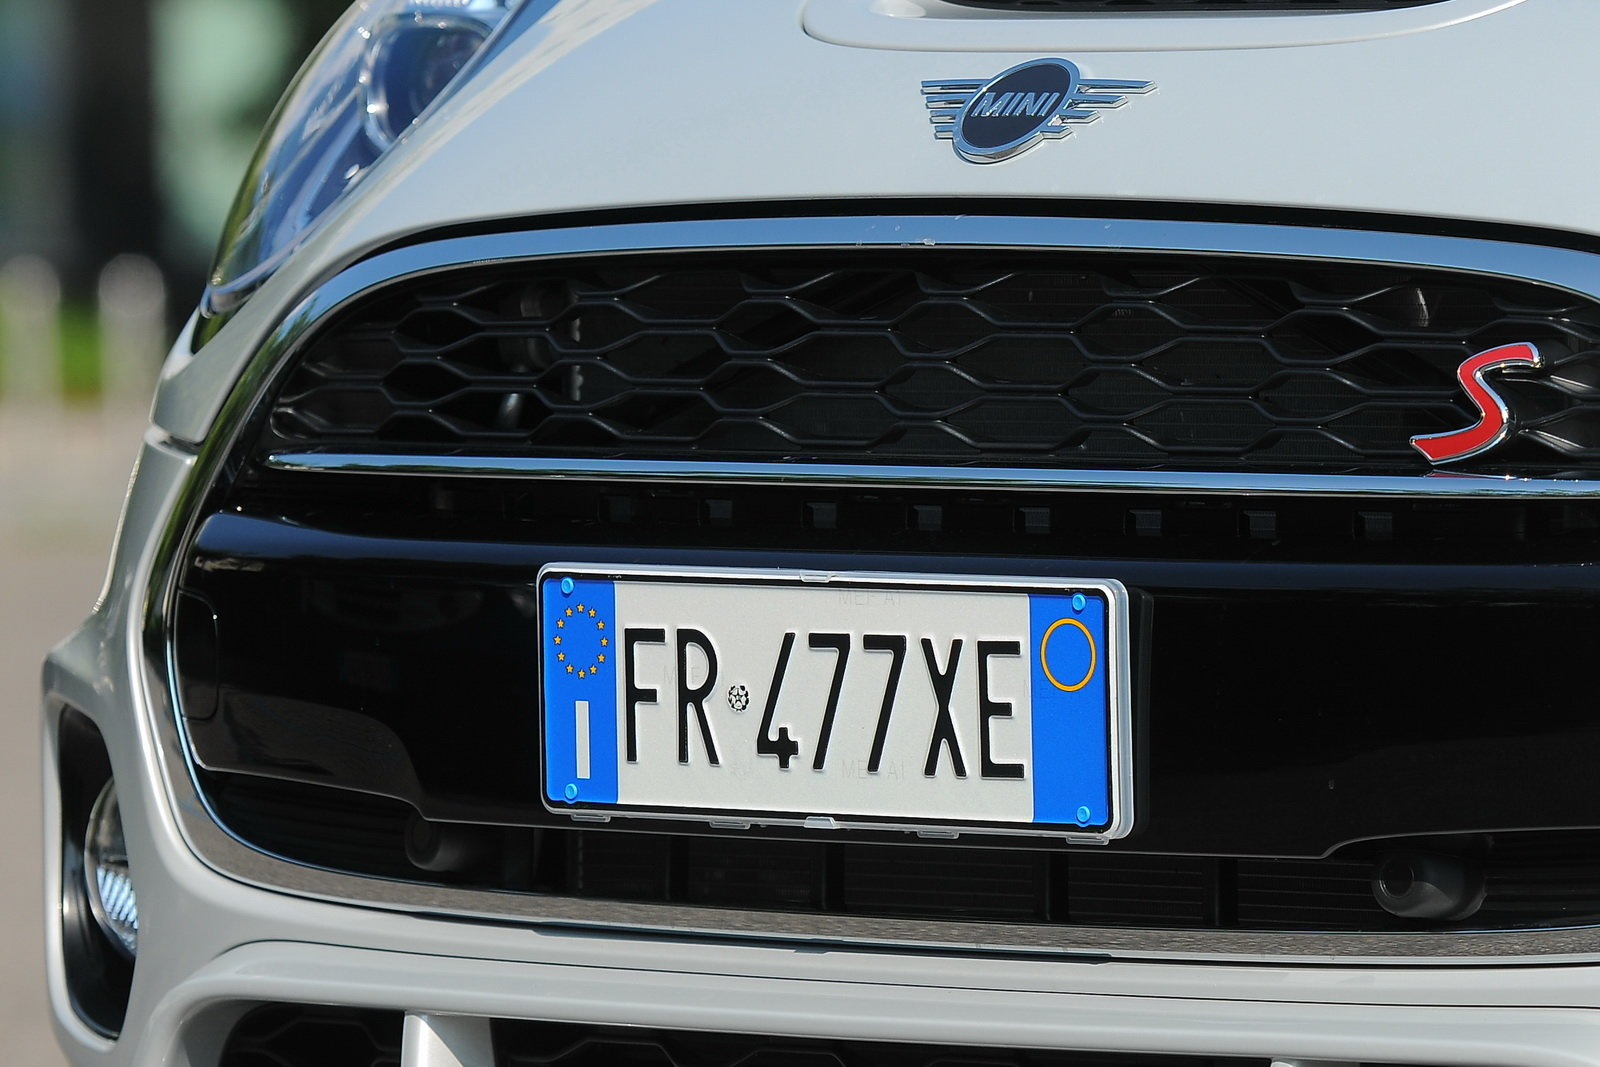
\includegraphics[width=3.5cm]{images/plate_23.jpg}\\[2pt]
            \scriptsize Immagine in ingresso\\
            \scriptsize $192 \times 192$ grayscale
        };
 
        % -------- BOX 2: Detection --------
        \node[stage, right=1.2cm of input] (det) {
            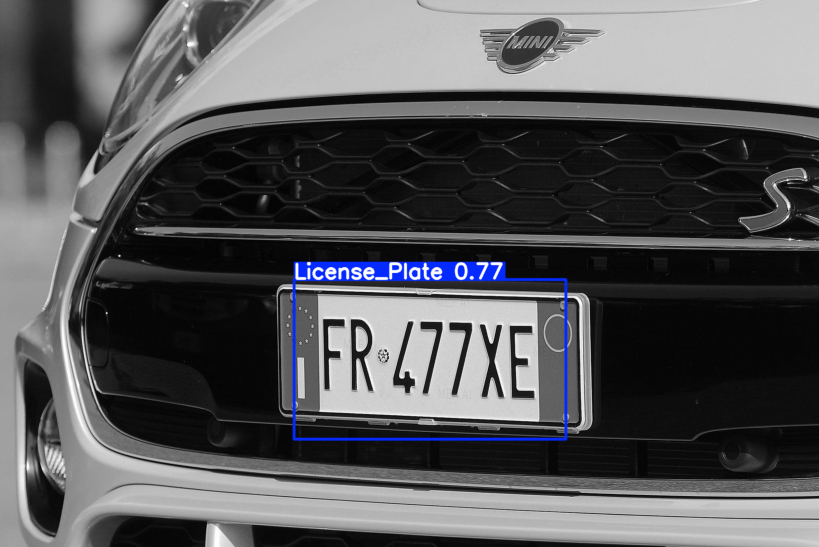
\includegraphics[width=3.5cm]{images/taega_boundingbox.png}\\[2pt]
            \scriptsize Detection (YOLO)\\
            \scriptsize bounding box della targa
        };
 
        % -------- BOX 3: OCR --------
        \node[stage, right=1.2cm of det] (ocr) {
            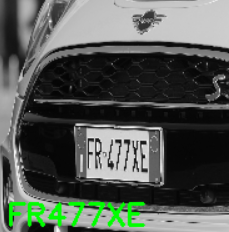
\includegraphics[width=3.0cm]{images/targa_esempio.png}\\[2pt]
            \scriptsize OCR (CCT-XS)\\
            \scriptsize testo decodificato
        };
 
        % -------- Frecce tra i box --------
        \draw[arrow] (input) -- node[above, label, custom_blue] {\tiny Stadio 1} (det);
        \draw[arrow] (det)   -- node[above, label, custom_blue] {\tiny Stadio 2} (ocr);
 
    \end{tikzpicture}
    \caption{Rappresentazione visiva della pipeline ALPR a due stadi.}
    \label{fig:pipeline-visiva}
\end{figure}


\section{Reti neurali per object detection: YOLO}
\label{sec:yolo}

Le reti neurali convoluzionali (\textit{Convolutional Neural Networks}, CNN) sono lo strumento standard per problemi di visione artificiale e si basano su uno schema gerarchico in cui ogni livello apprende rappresentazioni progressivamente più astratte a partire dai pixel grezzi. La famiglia di modelli YOLO (\textit{You Only Look Once})~\cite{redmon_2016_yolo} ha introdotto un approccio unificato al problema della detection: anziché applicare un classificatore su un insieme di proposte di regione, YOLO formula la detection come un unico problema di regressione, in cui una singola rete predice contemporaneamente posizioni e classi di tutti gli oggetti presenti nell'immagine.

La versione utilizzata in questo progetto è \textbf{YOLOv8}~\cite{jocher_2023_yolov8}, sviluppata e mantenuta da Ultralytics. Rispetto alle versioni precedenti, YOLOv8 introduce un \textit{backbone} basato su moduli C2f (Cross-Stage Partial con due flussi paralleli), un \textit{neck} di tipo PAN (\textit{Path Aggregation Network}) per la fusione di feature multi-scala, e una \textit{head} di tipo \textit{anchor-free} che predice direttamente le coordinate dei bounding box senza ricorrere a prior fissati. L'architettura è organizzata in tre uscite di rilevamento corrispondenti a tre scale spaziali differenti, consentendo di catturare oggetti di dimensioni eterogenee. Per ogni anchor della griglia di output, la rete predice quattro valori che descrivono il bounding box (centro e dimensioni) e un valore di confidenza per ciascuna classe. Nel caso di una rete a singola classe, come quella di questo progetto, l'output è dunque costituito da un tensore di forma $[1, 4, N]$ per i bounding box e $[1, 1, N]$ per le confidenze, dove $N$ è il numero totale di anchor che dipende dalle dimensioni dell'immagine in input.

\subsection{Non-Maximum Suppression}
\label{sec:nms}

Dopo l'inferenza, la rete restituisce tipicamente molte detection sovrapposte che si riferiscono allo stesso oggetto. La \textit{Non-Maximum Suppression} (NMS) è la procedura standard per ridurre tali duplicati a una singola predizione per oggetto. L'algoritmo seleziona la detection con confidenza massima e scarta tutte le altre che presentano un'\textit{Intersection over Union} (IoU) superiore a una soglia prefissata. L'IoU tra due bounding box $A$ e $B$ è definita come:
\[
\text{IoU}(A, B) = \frac{|A \cap B|}{|A \cup B|}
\]
e rappresenta il rapporto tra l'area di intersezione e quella di unione. Tipicamente si scartano box con IoU oltre $0{,}5$, ritenendo che facciano riferimento al medesimo oggetto.
\vspace{1.0cm}

\begin{figure}[H]
    \centering
    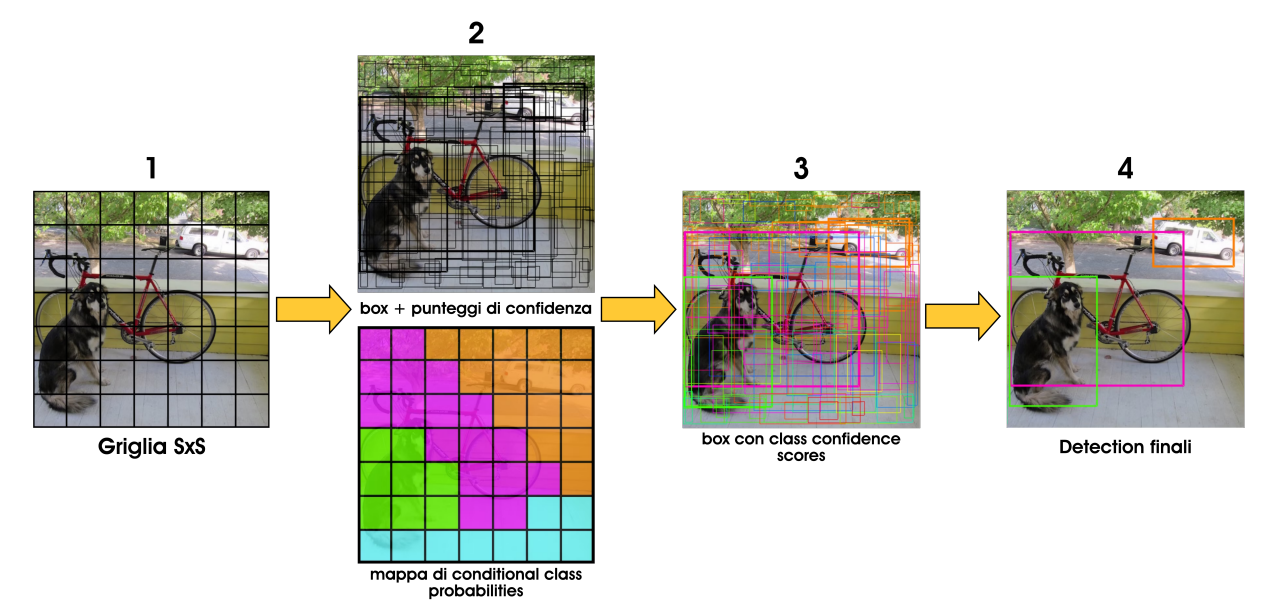
\includegraphics[width=1.0\textwidth]{images/inferenza_yolov8.png}
    \caption{Step della fase di inferenza nelle reti YOLO}
    \label{fig:inferenza yolov8}
\end{figure}


\newpage
\section{Vision Transformer e Compact Convolutional Transformer}
\label{sec:vit-cct}

\iffalse
I \textbf{Vision Transformer} (ViT) sono una classe di modelli che applica l'architettura Transformer, originariamente sviluppata per il \textit{Natural Language Processing}, al dominio delle immagini. L'idea di base è suddividere l'immagine in \textit{patch} non sovrapposte, proiettarle in uno spazio di embedding e processarle come una sequenza di token attraverso un meccanismo di \textit{self-attention} che permette a ciascun token di interagire con tutti gli altri.

Il vantaggio dei ViT rispetto alle CNN consiste nella capacità di modellare relazioni a lungo raggio direttamente, senza dipendere dalla gerarchia di livelli convoluzionali. Lo svantaggio principale è la necessità di grandi quantità di dati di addestramento, poiché il modello dispone di pochissimi bias induttivi (a differenza delle CNN, che hanno la \textit{translation invariance} integrata nella struttura). Inoltre, le architetture ViT originali richiedono milioni di parametri e sono difficilmente eseguibili su hardware con risorse limitate.

Per risolvere questi problemi, Hassani et al.~\cite{hassani_2021_cct} hanno proposto il \textbf{Compact Convolutional Transformer} (CCT), un'architettura ibrida che combina i vantaggi delle CNN e dei Transformer. Le differenze principali rispetto al ViT sono due. Anzitutto, l'embedding iniziale delle patch viene sostituito da un piccolo \textit{convolutional tokenizer}: alcuni strati convoluzionali estraggono feature locali dall'immagine e producono i token di ingresso del Transformer, restituendo a buon mercato i bias induttivi tipici delle CNN. In secondo luogo, il classificatore finale impiega un meccanismo di \textit{sequence pooling} che aggrega l'intera sequenza di token tramite attenzione, anziché utilizzare il token \texttt{[CLS]} dedicato come nel ViT originale.

Il risultato è un modello che mantiene la capacità rappresentazionale dei Transformer ma con un numero di parametri significativamente ridotto e una migliore efficienza di addestramento su dataset di dimensioni contenute. La variante \textbf{CCT-XS} utilizzata in questo progetto è la versione di scala più piccola della famiglia, particolarmente adatta a contesti embedded.
\fi

I \textbf{Vision Transformer} (ViT) applicano l'architettura Transformer, nata per il task di NLP, al dominio delle immagini, suddividendo l'immagine in patch e processandole come sequenze di token tramite \textit{self-attention}. Rispetto alle CNN, i ViT modellano relazioni a lungo raggio più efficacemente, ma richiedono grandi quantità di dati e molti parametri, risultando difficilmente adattabili a hardware con risorse limitate. Per ovviare a questi limiti, Hassani et al.~\cite{hassani_2021_cct} hanno proposto il \textbf{Compact Convolutional Transformer} (CCT), un'architettura ibrida che sostituisce l'embedding iniziale delle patch con un \textit{convolutional tokenizer} grazie al quale alcuni strati convoluzionali estraggono feature locali dall'immagine e producono i token di ingresso del Transformer. In secondo luogo, il classificatore finale impiega un meccanismo di \textit{sequence pooling} che aggrega l'intera sequenza di token tramite attenzione, anziché utilizzare il token \texttt{[CLS]} dedicato come nel ViT originale. Il risultato è un modello compatto, con un numero di parametri significativamente ridotto rispetto al ViT originale e una migliore efficienza di addestramento su dataset di dimensioni contenute.

Nel presente progetto, il CCT non è stato addestrato direttamente. La variante \texttt{CCT-XS}, la versione di scala più piccola della famiglia, è l'architettura alla base di una repository open-source individuata per il modulo OCR su targhe automobilistiche \cite{ankandrew_2024_fastplateocr}. Da essa sono stati ereditati sia i pesi pre-addestrati sul riconoscimento di caratteri sia la struttura di inferenza, che è stata successivamente adattata e quantizzata per il deployment sulla Board B. La scelta di questa architettura si è rivelata adeguata al contesto embedded grazie alle sue dimensioni contenute e alla buona accuratezza sul riconoscimento di sequenze alfanumeriche tipiche delle targhe automobilistiche.
\begin{figure}[H]
    \centering
    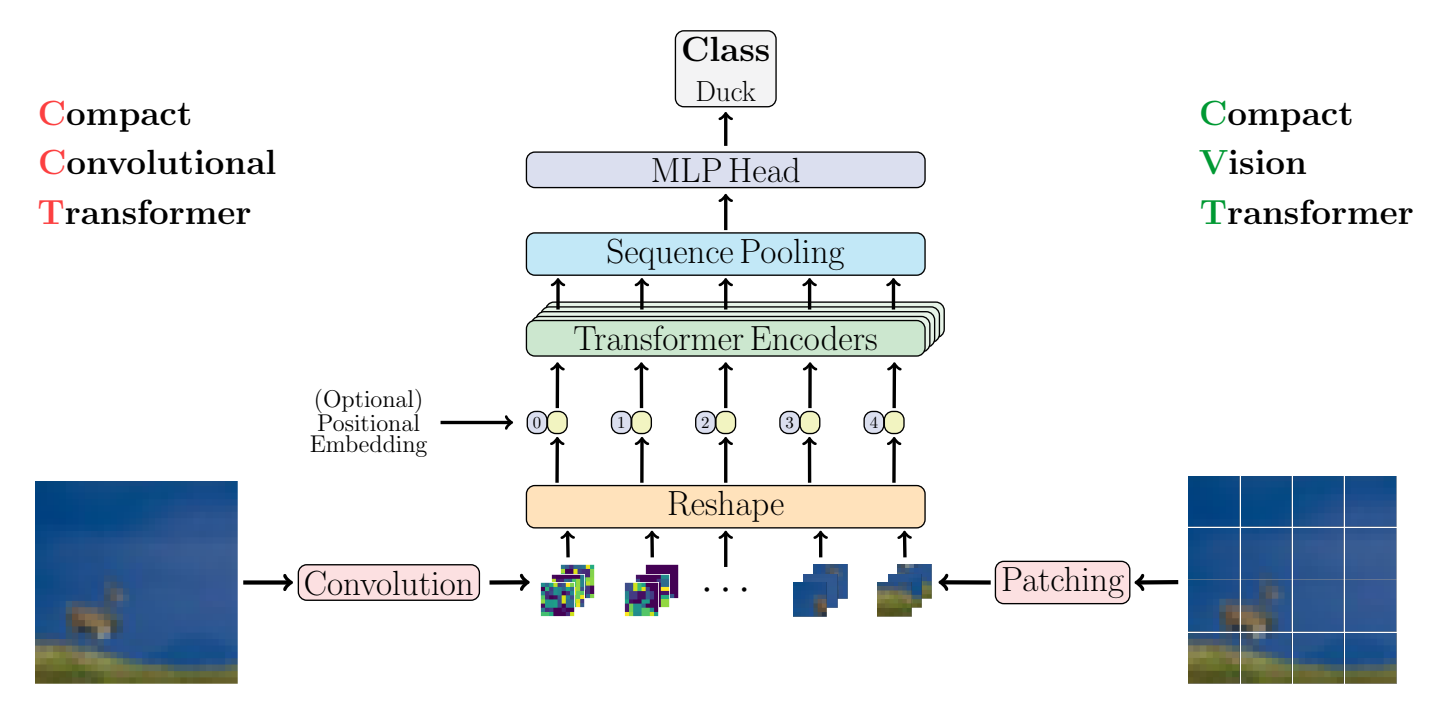
\includegraphics[width=0.9\textwidth]{images/cvtransofrmer.png}
    \caption{Architettura proposta nel paper "\textit{Escaping the Big Data Paradigm with
Compact Transformers}"}
    \label{fig:architettura-cct}
\end{figure}

\section{Quantizzazione INT8 e X-CUBE-AI}
\label{sec:quantization}

I modelli neurali sono tipicamente addestrati in aritmetica a virgola mobile a 32 bit (FP32). Tuttavia, per l'esecuzione su microcontrollori questo formato è inefficiente sia in termini di memoria (i pesi occupano 4 byte ciascuno) sia di prestazioni, perché molti microcontrollori non possiedono unità SIMD per il calcolo vettoriale in floating point. La tecnica della \textbf{quantizzazione} consiste nel rappresentare i pesi e le attivazioni della rete con interi a precisione ridotta, tipicamente 8 bit~\cite{jacob_2018_quantization}, riducendo l'occupazione di memoria di un fattore quattro e abilitando l'uso di istruzioni intere veloci.

\begin{boxH}
La quantizzazione INT8 con \textit{scale} e \textit{zero-point} è la forma più comune e mappa un valore reale $r$ su un intero $q$ a 8 bit tramite la relazione:
\textbf{\[
r = (q - z) \cdot s
\]}
\end{boxH}
dove $s$ (scale) è un fattore di scala in virgola mobile e $z$ (zero-point) è un offset intero. I parametri $s$ e $z$ vengono determinati separatamente per ciascun tensore della rete a partire da un piccolo insieme di campioni di calibrazione che permette di stimare l'intervallo dinamico dei valori. La conversione finale dell'output da intero a reale, detta \textit{dequantizzazione}, è dunque un'operazione esplicita che viene effettuata in software dopo l'inferenza, prima dell'applicazione di soglie o funzioni non lineari come la softmax.

In questo progetto la quantizzazione è affidata a \textbf{X-CUBE-AI} di STMicroelectronics~\cite{stm32cubeai_doc}, che importa il modello ONNX, applica la quantizzazione post-training e genera una libreria C ottimizzata per STM32. Il codice prodotto espone inoltre i parametri \texttt{SCALE} e \texttt{ZERO\_POINT}, necessari per quantizzare gli input e dequantizzare gli output dell'inferenza.

\section{Zephyr come sistema operativo embedded}
\label{sec:zephyr}

\textbf{Zephyr}~\cite{zephyr_doc} è un sistema operativo real-time open source pensato per dispositivi con risorse limitate. Nel progetto è stato scelto per la sua modularità, basata su KConfig e devicetree, che consente di includere solo i componenti necessari e di descrivere l'hardware in modo separato dal codice applicativo. Rispetto ad alternative come HAL o FreeRTOS, Zephyr offre driver già pronti e una configurazione più flessibile della piattaforma STM32H7. In particolare, sono risultati decisivi il supporto alla UART interrupt-driven, la possibilità di riconfigurare la SRAM tramite overlay devicetree e la compatibilità con la FPU hard-float richiesta dalla libreria X-CUBE-AI.

\begin{figure}[H]
    \centering
    
\includegraphics[width=0.3\textwidth]{images/logo_zephyt.png}
    \caption{Logo di \textit{Zephyr OS}.}
    \label{fig:zephyr os}
\end{figure}

\chapter{Architettura del sistema}
\label{cap:architettura}

Il sistema è organizzato come una pipeline distribuita su due microcontrollori indipendenti che comunicano via UART. Una terza unità, il PC host, ha il ruolo di sorgente delle immagini e di destinazione del risultato finale. Questo capitolo descrive la suddivisione dei compiti tra i tre nodi, la disposizione fisica dei collegamenti e le motivazioni che hanno guidato la scelta di un'architettura distribuita.

\section{Suddivisione dei compiti}
\label{sec:suddivisione}

Il flusso di elaborazione attraversa tre nodi in sequenza, ognuno responsabile di una fase specifica della pipeline ALPR:

\begin{itemize}
    \item Il \textbf{PC host} esegue lo script Python di test, che si occupa del pre-processing dell'immagine (conversione in scala di grigi e ridimensionamento a $192\times192$~pixel), dell'invio del payload al sistema embedded via UART e della visualizzazione del risultato finale. Il PC non partecipa all'inferenza.
    \item La \textbf{Board A} riceve l'immagine grayscale, ne calcola la quantizzazione INT8, esegue la rete YOLOv8-tiny per individuare la targa, applica la \textit{Non-Maximum Suppression} e ritaglia la porzione di immagine corrispondente. Questo viene quindi ridimensionato a $128\times64$~pixel tramite interpolazione \textit{nearest-neighbor}. Il crop così ottenuto viene inoltrato alla Board B e ne attende la risposta che viene successivamente mandata al PC.
    \item La \textbf{Board B} riceve il ritaglio in scala di grigi $128\times64$~pixel, lo espande sui tre canali RGB attesi dalla rete OCR, esegue il modello CCT-XS, decodifica la sequenza di logit in una stringa alfanumerica e la restituisce alla Board A.
\end{itemize}

La Figura~\ref{fig:flusso_nodi} riassume il flusso di dati e l'evoluzione del payload lungo la pipeline.

\begin{figure}[H]
    \centering
    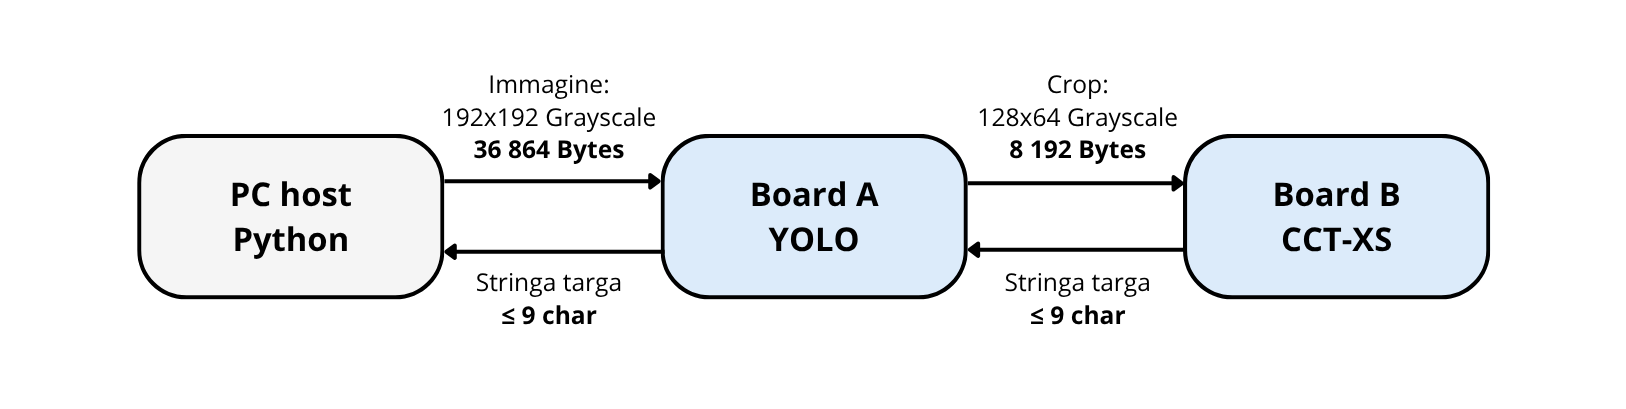
\includegraphics[width=1.1\textwidth]{images/flusso_nodi.png}
    \caption{Flusso dei dati tra i nodi lungo la pipeline}
    \label{fig:flusso_nodi}
\end{figure}

\newpage

\iffalse
\section{Motivazioni dell'architettura distribuita}
\label{sec:motivazioni}

La scelta di distribuire la pipeline su due microcontrollori, anziché eseguire entrambi i modelli su un singolo dispositivo, deriva da un vincolo concreto di memoria. Una stima preliminare ha mostrato che la sola rete YOLO occupa oltre 400~KB di RAM per le \textit{activation}, mentre la rete CCT-XS ne richiede circa 290~KB. La somma supera la capacità della SRAM principale della STM32H745, che è di 512~KB. Eseguire i due modelli sulla stessa unità avrebbe richiesto un meccanismo di scambio dei pesi tra Flash e RAM tra una fase e l'altra, oppure un'allocazione manuale su regioni di memoria diverse, con conseguente complessità implementativa e perdita di prestazioni.

Distribuire i due modelli su schede separate elimina questo problema alla radice: ciascuna scheda ospita un solo modello, dispone della totalità della propria SRAM per le activation e può essere programmata in modo indipendente. Il prezzo da pagare è la necessità di trasferire i dati tra le due schede attraverso un canale di comunicazione, scelta che però introduce contemporaneamente un caso d'uso didatticamente interessante --- la sincronizzazione tra microcontrollori --- coerente con gli obiettivi del corso di Sistemi Operativi Dedicati.
\fi

\section{Collegamenti hardware}
\label{sec:collegamenti}

Le due schede sono collegate al PC host e tra loro attraverso tre canali UART seriali, tutti operanti a 115\,200~baud con configurazione 8N1. La Figura~\ref{fig:schema_collegamenti} mostra lo schema fisico dei collegamenti tra le due schede STM, evidenziando le porte coinvolte e i pin del microcontrollore utilizzati per la comunicazione tra le board che è stata realizzata tramite l'interfaccia \textbf{USART2} collegando fisicamente i pin in modalità incrociata: il pin \textbf{PD5 (TX)} di ciascuna scheda è connesso al pin \textbf{PD6 (RX)} dell'altra, in modo che la trasmissione di una corrisponda alla ricezione dell'altra. È necessario inoltre collegare tra loro i pin \textbf{GND} delle due schede, in modo da stabilire un riferimento di tensione comune: poiché la comunicazione seriale UART è single-ended, il livello logico del segnale TX viene interpretato dalla scheda ricevente rispetto al proprio ground, e in assenza di una massa condivisa i livelli di tensione risulterebbero indefiniti, rendendo la comunicazione inaffidabile o del tutto impossibile.\\ 
Lato firmware, l'interfaccia è stata abilitata e configurata tramite il sistema di \textit{Device Tree overlay} di Zephyr RTOS, come visibile nel Listato \ref{lst:abilitazione_pin}. Questo approccio consente di separare nettamente la configurazione hardware dal codice applicativo, delegando al Device Tree la gestione dei mapping dei pin e dei parametri del bus.\\
\begin{lstlisting}[style=stileYAML, caption={Device Tree overlay per l'abilitazione dei pin PD5 e PD6}, label={lst:abilitazione_pin}]
&usart2 {
    status = "okay";
    current-speed = <115200>;
    pinctrl-0 = <&usart2_tx_pd5 &usart2_rx_pd6>;
    pinctrl-names = "default";
};
\end{lstlisting}
\begin{figure}[H]
    \centering
    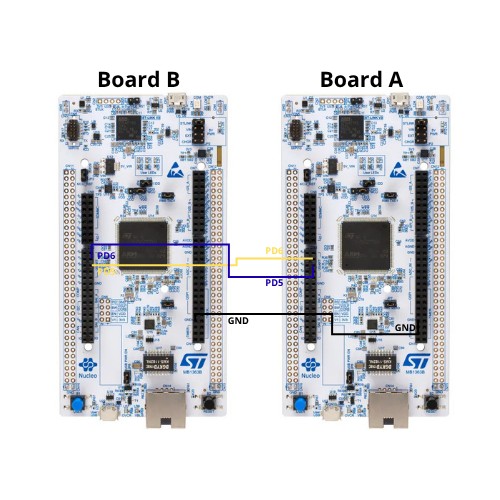
\includegraphics[width=0.55\textwidth]{images/immagine_collegamenti.png}
    \caption{Schema dei collegamenti tra le due Board}
    \label{fig:schema_collegamenti}
\end{figure}

Il collegamento tra il PC e la Board A sfrutta l'interfaccia \textbf{ST-Link} integrata sulla scheda Nucleo, che espone automaticamente un canale UART virtuale mappato sulla USART3 del microcontrollore. In questo modo il PC può inviare l'immagine da elaborare e ricevere il risultato del riconoscimento tramite una semplice comunicazione seriale, senza che il firmware debba gestire alcuno stack USB dedicato: la Board A interagisce con l'host esattamente come farebbe con qualsiasi altro dispositivo seriale. La Board B, invece, non dovendo comunicare direttamente con il PC, richiede unicamente l'alimentazione tramite cavo USB per essere operativa all'interno del sistema.\\
La Figura \ref{fig:setup} illustra il banco di prova allestito per la validazione del sistema, con evidenza dei collegamenti fisici realizzati tra le due schede e il PC.

\begin{figure}[H]
    \centering
    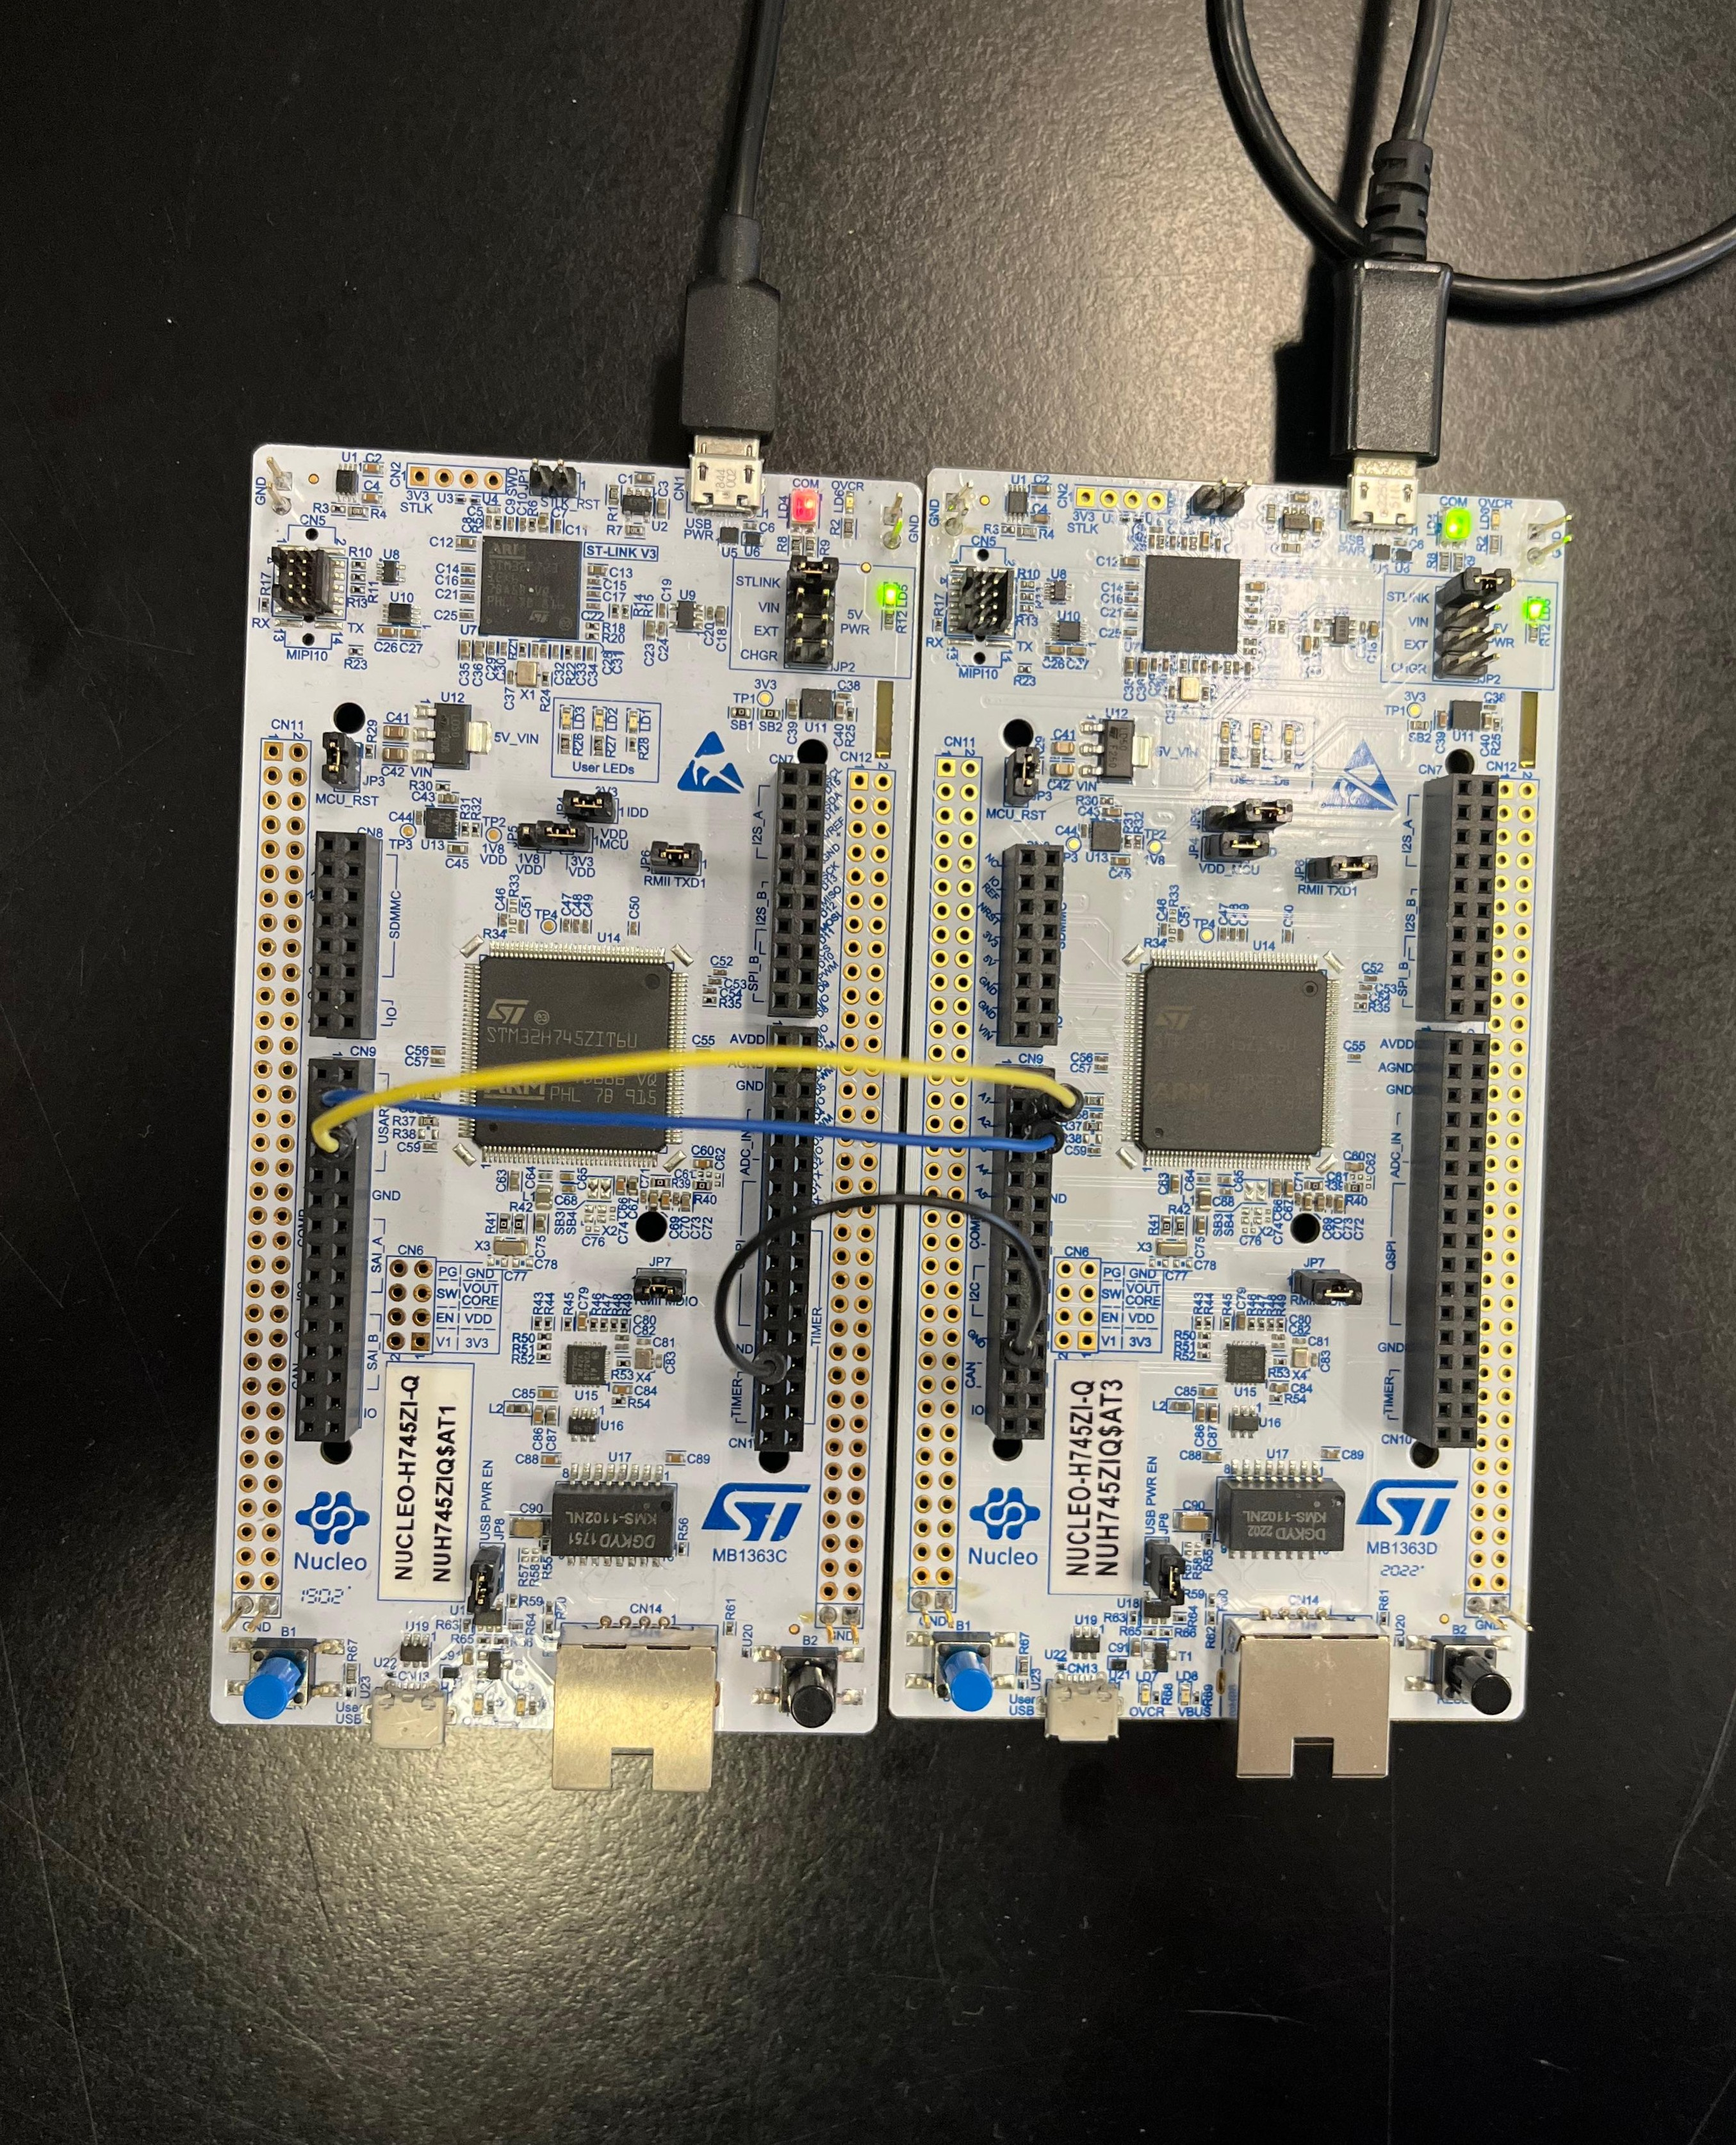
\includegraphics[width=0.7\textwidth]{images/setup_board.jpeg}
    \caption{Fotografia del banco di prova con le due schede collegate}
    \label{fig:setup}
\end{figure}


\chapter{Detection: Board A}
\label{cap:detection}

La Board A è responsabile del primo stadio della pipeline ALPR: a partire da un'immagine 192$\times$192 grayscale ricevuta dal PC, deve individuare la regione contenente la targa, ritagliarla e inoltrarla alla Board B per il riconoscimento dei caratteri. Questo capitolo descrive la rete neurale impiegata, il processo di addestramento, la validazione, l'esportazione del modello e l'implementazione del firmware Zephyr che lo integra.

\section{Rete YOLOv8-tiny custom}
\label{sec:yolov8t}

La rete utilizzata è una variante personalizzata di YOLOv8, ridotta in scala per adattarsi ai vincoli di memoria del microcontrollore. Il framework Ultralytics non prevede ufficialmente una scala più piccola della \texttt{n} (\textit{nano}); è stata quindi definita manualmente una nuova scala denominata \texttt{t} (\textit{tiny}), caratterizzata da un fattore di larghezza dei canali pari a $0{,}125$, esattamente la metà di quello di YOLOv8n, e da una profondità di $0{,}33$. Il file di configurazione della rete è stato inoltre modificato per accettare in ingresso immagini a singolo canale (\texttt{ch:~1}) e prevedere una singola classe (\texttt{nc:~1}), corrispondente all'etichetta \texttt{license\_plate}. La porzione rilevante del file di configurazione è riportata nel Listing~\ref{lst:yolo-yaml}.

\begin{lstlisting}[style=stileYAML, caption={Configurazione \texttt{yolov8t.yaml} che definisce la scala \texttt{t} a singolo canale e singola classe.}, label={lst:yolo-yaml}]
ch: 1
nc: 1
scales:
  t: [0.33, 0.125, 512]  # tiny: width 0.125 = meta di yolov8n


backbone:
  - [-1, 1, Conv, [64, 3, 2]]
  - [-1, 1, Conv, [128, 3, 2]]
  - [-1, 3, C2f, [128, True]]
  - [-1, 1, Conv, [256, 3, 2]]
  - [-1, 6, C2f, [256, True]]
  - [-1, 1, Conv, [512, 3, 2]]
  - [-1, 6, C2f, [512, True]]
  - [-1, 1, Conv, [1024, 3, 2]]
  - [-1, 3, C2f, [1024, True]]
  - [-1, 1, SPPF, [1024, 5]]

head:
  - [-1, 1, nn.Upsample, [None, 2, "nearest"]]
  - [[-1, 6], 1, Concat, [1]]
  - [-1, 3, C2f, [512]]
  - [-1, 1, nn.Upsample, [None, 2, "nearest"]]
  - [[-1, 4], 1, Concat, [1]]
  - ...
\end{lstlisting}

\section{Addestramento}
\label{sec:addestramento}

L'intero processo di addestramento è stato sviluppato su Google Colab utilizzando il framework Ultralytics, a partire dal dataset open source \textit{License-Plate-Recognition} (versione 4) pubblicato sulla piattaforma Roboflow Universe~\cite{roboflow_universe}. Il dataset contiene immagini di veicoli a colori con annotazioni dei bounding box delle targhe in formato YOLO, suddivise nei tre split di training, validation e test secondo la ripartizione predefinita dal pubblicatore.

\subsection{Preparazione del dataset}
\label{sec:dataset-prep}

Poiché la rete è progettata per accettare in ingresso immagini a singolo canale, è stato implementato uno script Python che converte in scala di grigi tutte le immagini dei tre split e aggiorna il file di configurazione \texttt{data.yaml} aggiungendo il parametro \texttt{channels:~1}, necessario per istruire Ultralytics sulla natura monocromatica dei dati. La conversione è parallelizzata su otto thread tramite \texttt{ThreadPoolExecutor} e gestisce in modo robusto eventuali file corrotti, rimuovendoli insieme alle relative etichette per non compromettere l'integrità del training.

\begin{lstlisting}[style=stilePython, caption={Conversione del dataset in scala di grigi.}, label={lst:gray-conversion}]
def converti_singola(img_path):
    try:
        img = Image.open(img_path).convert("L")
        img.save(img_path)
    except Exception:
        corrotte.append(img_path)
        img_path.unlink()

def converti_grayscale(dataset_path):
    for split in ["train", "valid", "test"]:
        img_dir = Path(dataset_path) / split / "images"
        images = list(img_dir.glob("*.jpg")) + \
                 list(img_dir.glob("*.jpeg")) + \
                 list(img_dir.glob("*.png"))
        with ThreadPoolExecutor(max_workers=8) as executor:
            executor.map(converti_singola, images)

# Aggiunta del campo channels nel data.yaml
data_info['channels'] = 1
\end{lstlisting}

\subsection{Configurazione e training}
\label{sec:train-config}

Il file di configurazione della rete è ottenuto a partire dal \texttt{yolov8.yaml} ufficiale di Ultralytics, modificato per introdurre la scala personalizzata \texttt{t} (\textit{tiny}) e per dichiarare il singolo canale in input e la singola classe in output. Una volta scritto su disco il file modificato, il modello viene istanziato direttamente dal file YAML senza partire da pesi pre-addestrati, perché la modifica del numero di canali in ingresso renderebbe incompatibili i pesi standard distribuiti per la versione RGB. L'addestramento è eseguito tramite il metodo \texttt{train()} dell'oggetto \texttt{YOLO}, con i parametri riportati sotto. I valori più significativi sono \texttt{epochs=50} (numero massimo di epoche), \texttt{patience=15} (\textit{early stopping} dopo 15 epoche senza miglioramenti), \texttt{imgsz=192} (risoluzione di ingresso fissata), \texttt{batch=64} (dimensione del batch), \texttt{lr0=0.01} (learning rate iniziale) e \texttt{pretrained=False} (training da zero per i motivi appena spiegati).

\begin{lstlisting}[style=stilePython, caption={Avvio dell'addestramento della rete YOLOv8-tiny custom.}, label={lst:training}]
model = YOLO(yaml_path)

results = model.train(
    data=f"{dataset.location}/data.yaml",
    epochs=50,
    imgsz=192,
    batch=64,
    patience=15,
    device=0,
    name="yolov8t_lp_gray",
    lr0=0.01,
    pretrained=False,
)
\end{lstlisting}

\subsection{Metriche di validazione}
\label{sec:metriche}

Al termine del training, il modello con i pesi migliori (\texttt{best.pt}) viene valutato sul set di validazione attraverso il metodo \texttt{val()} di Ultralytics. Le metriche ottenute sono riportate in Tabella~\ref{tab:yolo-metrics}. Il valore di mAP@0.5 di $0{,}941$ indica un'accuratezza elevata nel rilevamento delle targhe; il fatto che la precisione sia superiore al recall ($0{,}979$ contro $0{,}908$) suggerisce che la rete è leggermente conservativa, preferendo non emettere una detection piuttosto che produrre un falso positivo. Questo comportamento è preferibile nel contesto applicativo: una falsa detection inviata alla pipeline OCR genererebbe una stringa di output priva di significato, mentre l'assenza di detection produce una risposta esplicita di tipo \texttt{TYPE\_NONE} che l'utente sa interpretare.

\begin{table}[H]
    \centering
    \caption{Metriche di validazione del modello YOLOv8-tiny custom.}
    \label{tab:yolo-metrics}
    \begin{tabular}{lc}
        \toprule
        \textbf{Metrica} & \textbf{Valore} \\
        \midrule
        mAP@0.5         & $0{,}941$ \\
        mAP@0.5:0.95    & $0{,}638$ \\
        Precision       & $0{,}979$ \\
        Recall          & $0{,}908$ \\
        F1 score        & $0{,}942$ \\
        \bottomrule
    \end{tabular}
\end{table}

\section{Test della rete addestrata}
\label{sec:testing-rete}

La fase di test è stata eseguita ancora nell'ambiente Colab, sfruttando l'API di Ultralytics, per verificare in modo qualitativo il comportamento del modello prima di affrontare la quantizzazione INT8 e l'esecuzione embedded. Le immagini di test sono state pre-elaborate con la stessa procedura applicata al dataset di training: conversione in scala di grigi tramite il metodo \texttt{convert("L")} di PIL e mantenimento del formato originale. La fase di inferenza è effettuata invocando il metodo \texttt{predict()} del modello, passando il percorso della cartella contenente le immagini di test, una soglia di confidenza di $0{,}5$ e la stessa risoluzione di $192\times192$ utilizzata in addestramento (Listing~\ref{lst:predict}).

\begin{lstlisting}[style=stilePython, caption={Inferenza su un insieme di immagini di test tramite l'API Ultralytics.}, label={lst:predict}]
best_model = YOLO("runs/detect/yolov8t_lp_gray/weights/best.pt")

results = best_model.predict(
    source=str(test_dir),
    conf=0.5,
    imgsz=192,
    save=False,
    verbose=False
)

# Estrazione di statistiche per ciascuna immagine
for result in results:
    n_plates = len(result.boxes)
    for box in result.boxes:
        conf = box.conf.item()
        xyxy = box.xyxy[0].tolist()
        # ...
\end{lstlisting}

Per ciascuna immagine processata vengono estratte le coordinate del bounding box e il valore di confidenza associato, e l'immagine viene visualizzata con il rettangolo della detection sovrapposto attraverso il metodo \texttt{plot()} fornito da Ultralytics. La Figura~\ref{fig:test-results} mostra una selezione dei risultati ottenuti su un campione di immagini di test contenenti targhe di paesi diversi.

\begin{figure}[H]
    \centering
    \begin{subfigure}[t]{0.48\textwidth}
        \centering
        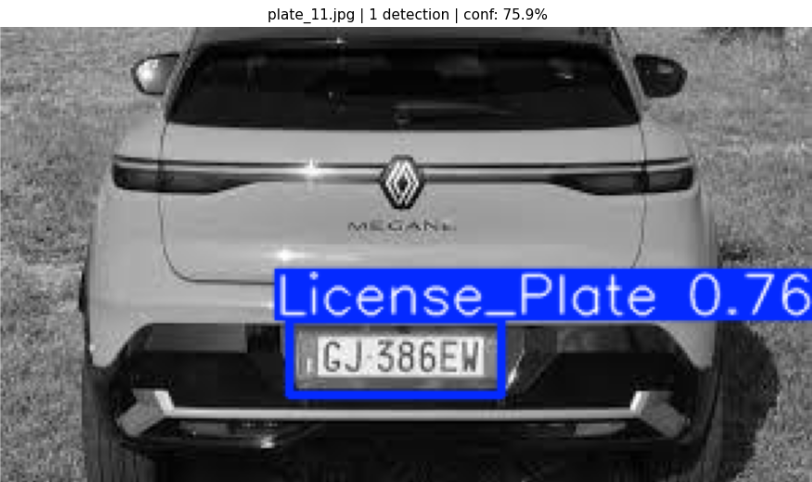
\includegraphics[width=0.80\textwidth]{images/yolov8t_test/plate_a.png}
        \label{fig:test-a}
    \end{subfigure}
    \hfill
    \begin{subfigure}[t]{0.48\textwidth}
        \centering
        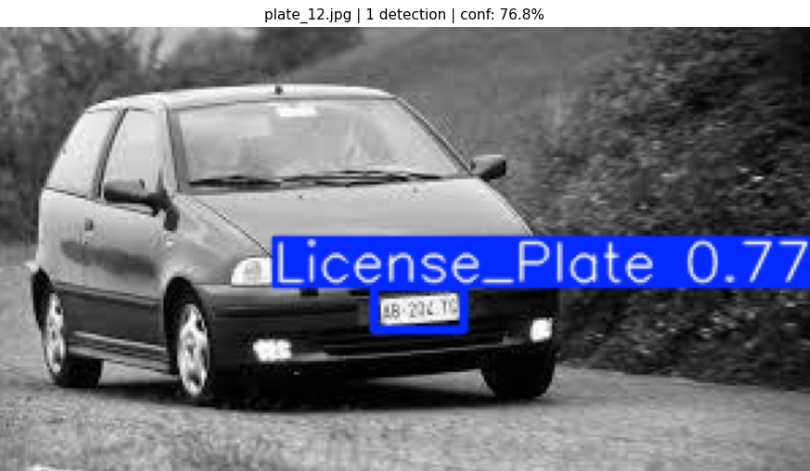
\includegraphics[width=0.80\textwidth]{images/yolov8t_test/plate_b.png}
        \label{fig:test-b}
    \end{subfigure}

    \vspace{0.4em}

    \begin{subfigure}[t]{0.48\textwidth}
        \centering
        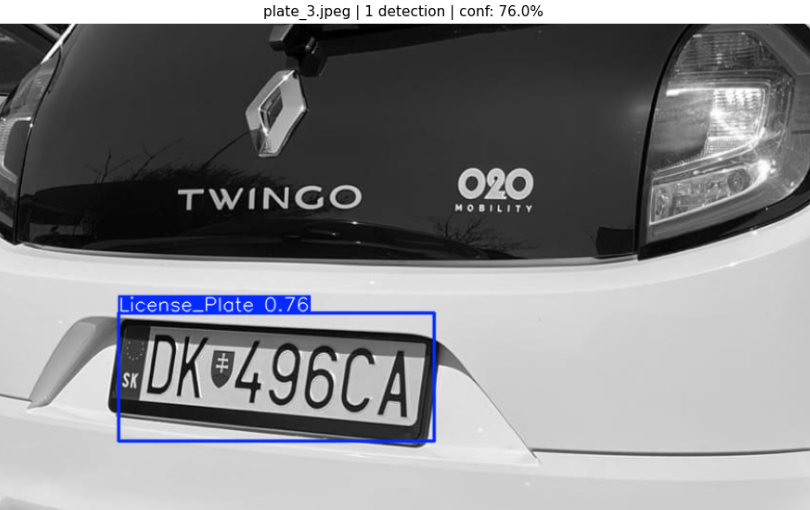
\includegraphics[width=0.80\textwidth]{images/yolov8t_test/plate_c.png}
        \label{fig:test-c}
    \end{subfigure}
    \hfill
    \begin{subfigure}[t]{0.48\textwidth}
        \centering
        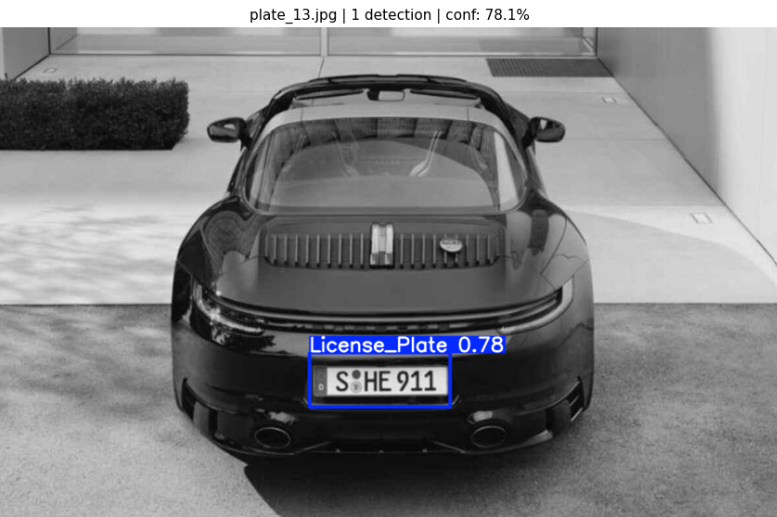
\includegraphics[width=0.80\textwidth]{images/yolov8t_test/plate_d.png}
        \label{fig:test-d}
    \end{subfigure}

    \caption{Esempi di output del modello YOLOv8-tiny custom su immagini di test.}
    \label{fig:test-results}
\end{figure}

I risultati di questa validazione preliminare hanno confermato che il modello generalizza correttamente su immagini esterne al dataset di addestramento, con confidenze tipicamente comprese tra $0{,}66$ e $0{,}96$ e un singolo caso di mancata detection in corrispondenza di un'immagine che non conteneva alcun veicolo.


%==============================================

\section{Esportazione ONNX e quantizzazione con X-CUBE-AI}
\label{sec:onnx-split}
 
Conclusa la fase di addestramento e validazione su Colab, il modello viene portato sul microcontrollore attraverso un processo a due passi: prima l'esportazione del file \texttt{best.pt} di Ultralytics in formato ONNX, poi l'importazione del file ONNX nello strumento X-CUBE-AI di STMicroelectronics che si occupa di quantizzare i pesi a INT8 e di generare la libreria C statica da linkare al firmware.
 
\subsection{Esportazione con output splittati}
\label{sec:export-split}
 
L'esportazione viene effettuata tramite l'API \texttt{export()} di Ultralytics con risoluzione di ingresso fissata a 192 e l'opzione \texttt{simplify=True}, che rimuove dal grafo i nodi ridondanti o di identità prodotti durante la conversione e ne agevola l'importazione in X-CUBE-AI. L'esportazione standard produce però un grafo che termina con un nodo \texttt{Concat} che combina i bounding box e le confidenze in un unico tensore di output di forma $[1, 5, 756]$. Questa rappresentazione è scomoda per il passo di quantizzazione successivo, perché i due flussi hanno intervalli di valori molto diversi: i bounding box assumono valori nell'intervallo $[0, 192]$ in coordinate pixel, mentre le confidenze sono limitate a $[0, 1]$. Forzare entrambi nello stesso tensore quantizzato in INT8 con un unico \textit{scale} comporterebbe una notevole perdita di precisione sulle confidenze, che si schiaccerebbero su pochi livelli di quantizzazione. Per questo motivo il nodo \texttt{Concat} finale è stato rimosso manipolando direttamente il grafo ONNX con la libreria \texttt{onnx}, e i due tensori intermedi (\texttt{boxes}, di forma $[1, 4, 756]$, e \texttt{conf}, di forma $[1, 1, 756]$) sono stati resi come output indipendenti. In questo modo X-CUBE-AI quantizza i due tensori con \textit{scale} e \textit{zero-point} separati, preservando la precisione di entrambi.
 
\subsection{Importazione in X-CUBE-AI}
\label{sec:cube-import}
 
X-CUBE-AI è il pacchetto di STMicroelectronics che importa modelli di reti neurali in formato ONNX, ne effettua la quantizzazione e ne genera una libreria C ottimizzata per la famiglia STM32 target. Il flusso di import è il medesimo per i due modelli del progetto e si articola in tre fasi:
 
\begin{enumerate}
    \item \textbf{Caricamento del modello}: il file ONNX viene importato nello strumento, che ne mostra le caratteristiche essenziali (dimensione dell'input, formato degli output, tipo dei dati).
    \item \textbf{Post-training quantization}: il flusso di quantizzazione è basato su ONNX Runtime e supporta sia una modalità con calibration dataset (un piccolo insieme di campioni in formato \texttt{.npz} che viene usato per stimare gli intervalli dinamici di pesi e attivazioni) sia una modalità con valori casuali, in cui gli intervalli vengono dedotti automaticamente. Nel progetto è stata scelta la modalità con valori casuali, accettando un'eventuale piccola degradazione di accuratezza in cambio di un flusso di lavoro più semplice e replicabile.
    \item \textbf{Ottimizzazione e generazione della libreria}: lo strumento offre tre profili di ottimizzazione:\textit{balanced}, \textit{RAM} e \textit{time}. Considerati i vincoli stringenti di memoria della STM32H745, è stato selezionato per entrambi i modelli il profilo \textit{optimization=ram}, che minimizza la dimensione dell'\textit{activation buffer} a scapito di un possibile leggero aumento del tempo di inferenza.
\end{enumerate}
 
\subsection{Risultati dell'ottimizzazione}
\label{sec:cube-results}
 
Al termine del passo di ottimizzazione, sul tool viene riportata una tabella riassuntiva con il numero di operazioni necessarie per una singola inferenza (MACC, \textit{Multiply-Accumulate operations}), l'occupazione di Flash distinta tra pesi e libreria runtime, e l'occupazione di RAM distinta tra \textit{activation buffer} e contesto della libreria. La Figura~\ref{fig:cube-stats} mostra l'output ottenuto per i due modelli e la Tabella~\ref{tab:cube-stats} ne riassume i numeri.
 
\begin{figure}[H]
    \centering
    \begin{subfigure}[t]{\textwidth}
        \centering
        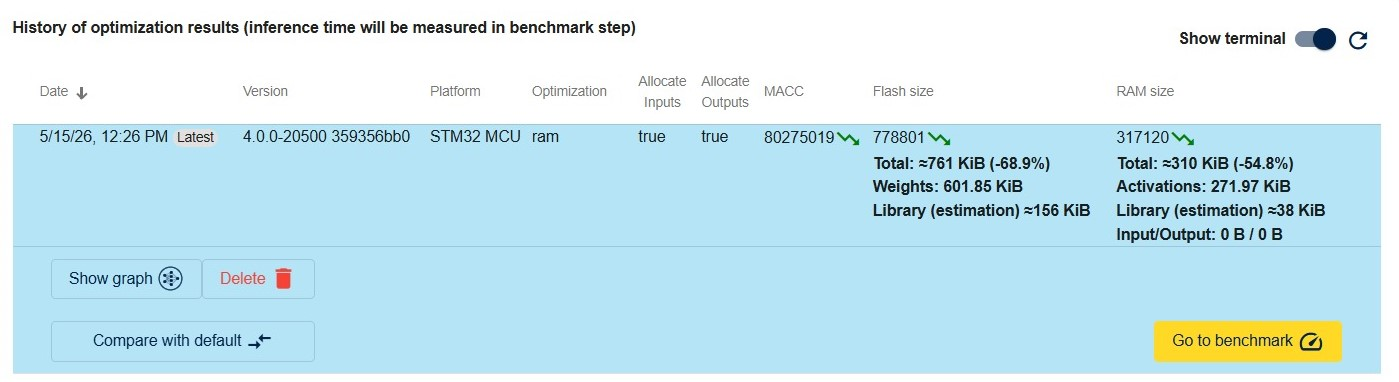
\includegraphics[width=0.90\textwidth]{images/xcubeai/xcubeai_a.jpeg}
        \caption{Risultati dell'ottimizzazione del detector YOLO con profilo \textit{ram}.}
        \label{fig:opt-yolo}
    \end{subfigure}
 
    \vspace{0.5em}
 
    \begin{subfigure}[t]{\textwidth}
        \centering
        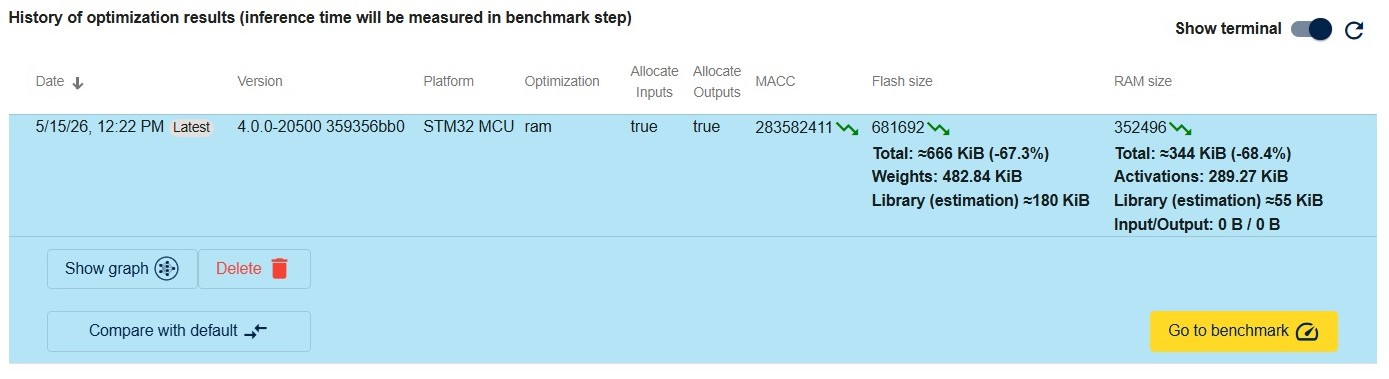
\includegraphics[width=0.90\textwidth]{images/xcubeai/xcubeai_b.jpeg}
        \caption{Risultati dell'ottimizzazione dell'OCR CCT-XS con profilo \textit{ram}.}
        \label{fig:opt-cct}
    \end{subfigure}
    \caption{Output di X-CUBE-AI al termine del passo di ottimizzazione per i due modelli.}
    \label{fig:cube-stats}
\end{figure}
 
\begin{table}[H]
    \centering
    \caption{Stima di occupazione di memoria e di operazioni prodotta da X-CUBE-AI per i due modelli quantizzati con profilo \textit{optimization=ram}.}
    \label{tab:cube-stats}
    \begin{tabular}{lrr}
        \toprule
        \textbf{Voce} & \textbf{YOLOv8-tiny} & \textbf{CCT-XS} \\
        \midrule
        MACC (per inferenza)             & 80\,275\,019 & 283\,582\,411 \\
        Flash totale stimata             & $\sim$761~KiB & $\sim$666~KiB \\
        \hspace{1em}Pesi                 & 601{,}85~KiB & 482{,}84~KiB \\
        \hspace{1em}Libreria runtime     & $\sim$156~KiB & $\sim$180~KiB \\
        RAM totale stimata               & $\sim$310~KiB & $\sim$344~KiB \\
        \hspace{1em}Activation buffer    & 271{,}97~KiB & 289{,}27~KiB \\
        \hspace{1em}Libreria runtime     & $\sim$38~KiB & $\sim$55~KiB \\
        \bottomrule
    \end{tabular}
\end{table}
 
%==============================================

\section{Integrazione nel firmware}
\label{sec:firmware-A}

Il firmware della Board A è organizzato come un singolo thread principale che esegue ciclicamente le fasi di ricezione, inferenza e invio. Le strutture dati allocate staticamente sono progettate per minimizzare l'occupazione di RAM e sono riassunte in Tabella~\ref{tab:buffer-A}.

\begin{table}[H]
    \centering
    \caption{Allocazione statica della RAM nel firmware di Board A.}
    \label{tab:buffer-A}
    \begin{tabular}{lrl}
        \toprule
        \textbf{Buffer} & \textbf{Dimensione} & \textbf{Funzione} \\
        \midrule
        \texttt{io\_buf} (union)   & 36\,864 B   & Immagine in input e tensore quantizzato \\
        \texttt{act\_buf}          & 410\,112 B  & Attivazioni intermedie della rete \\
        \texttt{out\_boxes}        & 3\,024 B    & Output: $4 \times 756$ INT8 \\
        \texttt{out\_conf}         & 756 B       & Output: $1 \times 756$ INT8 \\
        \texttt{net\_ctx}          & --          & Contesto della libreria X-CUBE-AI \\
        \texttt{crop\_buf}         & 8\,196 B    & Crop $128 \times 64$ + header \\
        \texttt{rx\_rb\_pc}        & 8\,192 B    & Ring buffer UART verso PC \\
        \texttt{rx\_rb\_b2b}       & 256 B       & Ring buffer UART verso Board B \\
        \bottomrule
    \end{tabular}
\end{table}

La scelta più importante in termini di occupazione di RAM è l'uso di una \texttt{\textbf{union}} per condividere fisicamente la stessa regione di memoria tra l'immagine ricevuta dal PC e l'input quantizzato della rete. Come mostrato nel Listing~\ref{lst:union-A}, i due membri della union (\texttt{gray} a 8 bit unsigned e \texttt{net\_in} a 8 bit signed) hanno la stessa dimensione e non vengono mai usati simultaneamente: l'immagine viene prima ricevuta nella forma a 8 bit unsigned, poi convertita in-place in INT8 sottraendo $128$ a ogni pixel.

\begin{lstlisting}[style=stileC, caption={Union per la condivisione del buffer di ingresso tra l'immagine ricevuta e il tensore quantizzato. Risparmia $36\,864$ byte di RAM.}, label={lst:union-A}]
static union {
    uint8_t gray[GRAY_SIZE];
    int8_t  net_in[STAI_NETWORK_IN_1_SIZE];
} io_buf __attribute__((aligned(4)));
\end{lstlisting}



\subsection{Quantizzazione in-place}
\label{sec:quant-A}

La quantizzazione viene effettuata con un semplice ciclo che traduce ogni pixel dal range $[0, 255]$ di tipo \texttt{uint8\_t} al range $[-128, 127]$ di tipo \texttt{int8\_t}, sottraendo $128$. Lo \textit{zero-point} è quindi pari a $128$ e la \textit{scale} è $1{,}0$: la rete è stata calibrata in modo da accettare direttamente i pixel grezzi, senza ulteriori normalizzazioni.

\begin{lstlisting}[style=stileC, caption={Quantizzazione.}, label={lst:quantization}]
// Quantizzazione
for (int i = 0; i < STAI_NETWORK_IN_1_SIZE; i++)
    io_buf.net_in[i] = (int8_t)((int)io_buf.gray[i] - 128);
\end{lstlisting}

\subsection{Parsing dell'output e NMS}
\label{sec:nms-A}

Dopo l'inferenza, gli output della rete vengono dequantizzati con la formula $r = (q - z) \cdot s$, usando i parametri \texttt{scale} e \texttt{zero\_point} generati da X-CUBE-AI. La routine \texttt{parse\_output} analizza le $756$ anchor, conserva solo le candidate con confidenza superiore a $0{,}5$ e seleziona quella con confidenza massima. Su queste candidate viene poi applicata una NMS semplificata: le detection con IoU superiore a $0{,}5$ rispetto alla migliore vengono scartate. Poiché il caso d'uso prevede al massimo una targa per immagine, il risultato finale coincide normalmente con il bounding box più affidabile, mantenendo comunque una maggiore robustezza in presenza di più rilevamenti.

\subsection{Costruzione del crop}
\label{sec:crop}

Prima del ritaglio il firmware ripristina i pixel originali sommando $128$ a
ciascun byte INT8 (operazione inversa della quantizzazione), poiché la
\texttt{union} \texttt{io\_buf} è stata sovrascritta in-place durante
l'inferenza. Il bounding box viene poi espanso di 5 pixel su ogni lato e
le coordinate sono clampate ai bordi dell'immagine per evitare accessi
fuori buffer. La regione risultante è ridimensionata a $128\times64$~pixel
con interpolazione \textit{nearest-neighbor}\footnote{L'interpolazione \textit{nearest-neighbor} (o \textit{nearest neighbour}) è una tecnica di ridimensionamento delle immagini in cui ogni nuovo pixel assume il valore del pixel originale più vicino. Il metodo non introduce operazioni di media o filtraggio ed è quindi particolarmente efficiente dal punto di vista computazionale.} e inviata alla Board B come frame
\texttt{TYPE\_CROP} preceduto da un header di 4 byte con le dimensioni.

\begin{figure}[H]
    \centering
    \begin{tikzpicture}[
        font=\footnotesize,
        % --- stile dei blocchi RAM ---
        ram/.style={
            draw, thick, minimum height=0.9cm, minimum width=8cm,
            align=center, font=\small
        },
        gray_box/.style={ram, fill=custom_lightgray},
        int8_box/.style={ram, fill=custom_lightblue},
        % --- stile delle frecce di transizione ---
        trans/.style={->, >=stealth, very thick, custom_blue},
        % --- etichetta laterale ---
        sidelbl/.style={font=\scriptsize\itshape, custom_gray, anchor=west},
        timelbl/.style={font=\scriptsize\bfseries, custom_red, anchor=east}
    ]

    % =================================================================
    % (a) Tre stati della stessa zona di RAM
    % =================================================================

    % --- Stato 1: dopo ricezione UART ---
    \node[timelbl] (t1) at (-0.3, 0)  {t = 1};
    \node[gray_box, right=0.1cm of t1] (s1) {
        \texttt{io\_buf.gray[]} \;--\; \texttt{uint8\_t} \;--\; pixel $\in [0, 255]$
    };
    \node[sidelbl, right=0.2cm of s1] {dopo ricezione UART};

    % --- Stato 2: dopo quantizzazione ---
    \node[timelbl, below=1.1cm of t1] (t2) {t = 2};
    \node[int8_box, right=0.1cm of t2] (s2) {
        \texttt{io\_buf.net\_in[]} \;--\; \texttt{int8\_t} \;--\; pixel $\in [-128, 127]$
    };
    \node[sidelbl, right=0.2cm of s2] {input quantizzato alla rete};

    % --- Stato 3: dopo inferenza, riconvertita ---
    \node[timelbl, below=1.1cm of t2] (t3) {t = 3};
    \node[gray_box, right=0.1cm of t3] (s3) {
        \texttt{io\_buf.gray[]} \;--\; \texttt{uint8\_t} \;--\; pixel $\in [0, 255]$
    };
    \node[sidelbl, right=0.2cm of s3] {pronto per il crop};

    % --- Frecce di transizione tra i 3 stati ---
    \draw[trans] (s1) -- node[right, font=\scriptsize, custom_blue, align=left]
        {\textbf{quantizzazione}\\$q = g - 128$} (s2);
    \draw[trans] (s2) -- node[right, font=\scriptsize, custom_blue, align=left]
        {\textbf{inferenza + dequant inversa}\\$g = q + 128$} (s3);

    % --- Annotazione "stesso indirizzo di memoria" sul lato sinistro ---
    \draw[thick, custom_red, decorate,
          decoration={brace, amplitude=6pt, mirror}]
        ($(t1.north west)+(-0.1, 0.1)$) -- ($(t3.south west)+(-0.1, -0.1)$);
    \node[custom_red, font=\scriptsize\bfseries, rotate=90, anchor=south]
        at ($(t2.west)+(-0.7, 0)$) {stessa zona di RAM (36\,864 B)};

    % =================================================================
    % (b) Confronto barra RAM: con union vs senza
    % =================================================================

    \node[font=\small\bfseries, below=1cm of s3, anchor=north]
        (label_bar) {Risparmio di RAM};

    % Posizione di partenza barre
    \coordinate (bar_origin) at ($(label_bar.south)+(0, -0.5)$);

    % --- Barra "Senza union" (2 buffer separati = 73 728 B) ---
    \node[anchor=east, font=\scriptsize] at ($(bar_origin)+(-3.6, 0)$)
        {Senza \texttt{union}:};
    \fill[custom_orange] ($(bar_origin)+(-3.5, -0.25)$)
        rectangle ($(bar_origin)+(3.5, 0.25)$);
    \node[font=\scriptsize, white, anchor=center]
        at ($(bar_origin)+(0, 0)$) {\textbf{73\,728 B} (gray + net\_in)};

    % --- Barra "Con union" (1 buffer = 36 864 B) ---
    \node[anchor=east, font=\scriptsize] at ($(bar_origin)+(-3.6, -0.8)$)
        {Con \texttt{union}:};
    \fill[custom_green] ($(bar_origin)+(-3.5, -1.05)$)
        rectangle ($(bar_origin)+(0, -0.55)$);
    \node[font=\scriptsize, white, anchor=center]
        at ($(bar_origin)+(-1.75, -0.8)$) {\textbf{36\,864 B}};

    \end{tikzpicture}

    \caption{Funzionamento della \texttt{union} nel firmware di Board A.}
    \label{fig:union-memoria}
\end{figure}
\chapter{OCR: Board B}
\label{cap:ocr}

La Board B esegue il secondo stadio della pipeline. A partire dal ritaglio della targa prodotto da Board A, una rete di tipo Compact Convolutional Transformer estrae il contenuto alfanumerico e lo restituisce come stringa di caratteri. A differenza della Board A, qui non c'è un addestramento personalizzato: si è scelto di utilizzare un modello pre-addestrato di alta qualità già disponibile pubblicamente, adattandone soltanto l'integrazione nel contesto embedded.

\section{Modello CCT-XS pre-addestrato}
\label{sec:cct-xs}

Il modello impiegato è \texttt{cct\_xs\_v1\_global}, distribuito nel repository open source\cite{ankandrew_2024_fastplateocr} mantenuto da ankandrew. Si tratta di una versione \textit{compact} di Vision Transformer (Sezione~\ref{sec:vit-cct}), addestrata specificamente per la lettura di targhe automobilistiche su un dataset multi-paese di grandi dimensioni. Come già discusso la scelta è motivata dal buon compromesso tra dimensioni e accuratezza: la variante \texttt{XS} occupa circa $500$~KB, generalizza su targhe di paesi diversi ed è già disponibile in formato ONNX, quindi può essere importata direttamente in X-CUBE-AI senza ulteriori passaggi da PyTorch. L'addestramento del modello non è stato ripetuto: la rete è utilizzata così com'è fornita dal repository, dopo la sola quantizzazione INT8 effettuata in fase di importazione.

\subsection{Formato di input e output}
\label{sec:io-cct}

Il modello accetta in ingresso un tensore di forma $[1, 64, 128, 3]$: un'immagine di altezza 64 e larghezza 128 con tre canali RGB. Il fatto che la rete sia stata addestrata su immagini a colori, mentre il flusso del progetto opera in scala di grigi, è gestito dal firmware con un'espansione triviale del canale grigio sui tre canali. L'output è un tensore di forma $[1, 9, 37]$, interpretato come una matrice di logit: ciascuno dei 9 \textit{slot} corrispondenti ai 9 caratteri della targa contiene un vettore di 37 punteggi, uno per ciascuna classe dell'alfabeto. L'alfabeto è composto dalle 10 cifre, dalle 26 lettere maiuscole e dal carattere speciale \texttt{\_} che funge da padding per indicare uno slot non utilizzato.

\begin{lstlisting}[style=stileC, caption={Alfabeto del modello OCR.}, label={lst:alphabet}]
// Dimensioni dell'immagine
#define IMG_W        128
#define IMG_H         64
#define GRAY_SIZE    (IMG_W * IMG_H)   // 8192 byte che arriva via UART
#define MSG_HEADER_SIZE  7

// Parametri OCR
#define NUM_SLOTS    9     
#define NUM_CLASSES  37   
static const char ALPHABET[NUM_CLASSES] = "0123456789ABCDEFGHIJKLMNOPQRSTUVWXYZ_";
\end{lstlisting}

\section{Integrazione nel firmware}
\label{sec:firmware-B}

L'architettura del firmware della Board B è più semplice di quella di Board A perché c'è un solo canale UART da gestire e un solo modello da eseguire. Anche qui tutte le strutture dati sono allocate staticamente; il prospetto è riportato in Tabella~\ref{tab:buffer-B}.

\begin{table}[H]
    \centering
    \caption{Allocazione statica della RAM nel firmware di Board B.}
    \label{tab:buffer-B}
    \begin{tabular}{lrl}
        \toprule
        \textbf{Buffer} & \textbf{Dimensione} & \textbf{Funzione} \\
        \midrule
        \texttt{io\_buf} (union)   & 24\,576 B   & Crop grayscale e tensore RGB \\
        \texttt{act\_buf}          & 296\,212 B  & Attivazioni intermedie della rete \\
        \texttt{out\_ocr}          & 333 B       & Output: $9 \times 37$ INT8 \\
        \texttt{net\_ctx}          & --          & Contesto della libreria X-CUBE-AI \\
        \texttt{rx\_rb}            & 8\,199 B    & Ring buffer UART verso Board A \\
        \bottomrule
    \end{tabular}
\end{table}

\subsection{Gray to RGB in-place}
\label{sec:rgb-expansion}

L'espansione del canale grigio in tre canali RGB è realizzata in-place sulla stessa union che ospita sia il payload ricevuto (\texttt{gray}, 8\,192 byte) sia l'input della rete (\texttt{net\_in}, 24\,576 byte). Per non sovrascrivere i pixel ancora da espandere, il ciclo procede dal fondo verso l'inizio del buffer, come mostrato nel Listato~\ref{lst:rgb-expand}. Ciascun pixel grigio viene copiato in tre posizioni consecutive del nuovo buffer.

\begin{lstlisting}[
    style=stileC,
    caption={Gray to RGB in-place. Il ciclo scorre i pixel dall'ultimo al primo per non sovrascrivere i dati ancora da convertire.},
    label={lst:rgb-expand}
]
// Ricezione crop da Board A (GRAY_SIZE byte)
if (recv_msg_b2b(&type, io_buf.gray, GRAY_SIZE, &len) != 0) {
    uint8_t e = 0x02;
    send_msg_b2b(TYPE_ERR, &e, 1);
    continue;
}

if (type != TYPE_CROP || len != GRAY_SIZE) {
    uint8_t e = 0x03;
    send_msg_b2b(TYPE_ERR, &e, 1);
    continue;
}

// Espansione gray -> RGB in-place
// (dal fondo per non sovrascrivere)
for (int i = GRAY_SIZE - 1; i >= 0; i--) {
    uint8_t g = io_buf.gray[i];

    io_buf.net_in[i * 3 + 0] = g;  // R
    io_buf.net_in[i * 3 + 1] = g;  // G
    io_buf.net_in[i * 3 + 2] = g;  // B
}
\end{lstlisting}

Questo accorgimento permette di evitare un secondo buffer da $24\,576$ byte e contribuisce in modo significativo al rispetto del budget di RAM disponibile.

\subsection{Decoding dell'output}
\label{sec:decoding}

La traduzione dei logit in stringa è un classico \textit{greedy decoding}\footnote{Il \textit{greedy decoding} è una strategia di decodifica in cui, ad ogni passo, viene selezionata la classe con probabilità (o logit) massima indipendentemente dalle altre possibili sequenze. Pur non garantendo la sequenza globalmente ottimale, è estremamente efficiente dal punto di vista computazionale ed è adatta a problemi in cui le predizioni dei singoli slot possono essere considerate indipendenti.} per ciascuno slot indipendentemente. La routine \texttt{decode\_plate} (Listato~\ref{lst:decode}) scorre gli slot da sinistra a destra, calcola per ciascuno l'argmax sulle 37 classi e accoda il carattere corrispondente alla stringa di output. La decodifica si interrompe non appena viene incontrato il carattere di padding \texttt{\_}, che segnala la fine della targa: questa scelta riflette il fatto che la rete è stata addestrata a produrre il padding solo dopo l'ultimo carattere significativo, mai in mezzo a una sequenza valida.

\begin{lstlisting}[style=stileC, caption={Decodifica della stringa di targa dai logit dell'OCR. Per ogni slot, si seleziona la classe con punteggio massimo; la decodifica si arresta al primo carattere di padding.}, label={lst:decode}]
static int decode_plate(char *out_str)
{
    int n_chars = 0;
    for (int slot = 0; slot < NUM_SLOTS; slot++) {
        int   best_cls   = 0;
        float best_score = -1e9f;
        for (int cls = 0; cls < NUM_CLASSES; cls++) {
            float score = dequant_ocr(out_ocr[slot * NUM_CLASSES + cls]);
            if (score > best_score) {
                best_score = score;
                best_cls = cls;
            }
        }
        if (ALPHABET[best_cls] == '_') break;
        out_str[n_chars++] = ALPHABET[best_cls];
    }
    out_str[n_chars] = '\0';
    return n_chars;
}
\end{lstlisting}

La dequantizzazione è effettuata sui 333 valori INT8 del tensore di output applicando i parametri di \textit{scale} ($\approx 0{,}00392$, ovvero $1/255$) e \textit{zero-point} ($-128$) generati da X-CUBE-AI. Si noti che, ai fini dell'argmax, la dequantizzazione non è strettamente necessaria: poiché la trasformazione è monotona, il massimo dei logit dequantizzati coincide con il massimo dei logit quantizzati. La dequantizzazione esplicita è mantenuta per chiarezza e per permettere eventuali estensioni future, come l'applicazione di una soglia sui punteggi.

\chapter{Comunicazione e protocollo}
\label{cap:comunicazione}

La comunicazione tra i tre nodi del sistema (PC, Board A e Board B) avviene esclusivamente attraverso canali UART seriali. Questo capitolo descrive il protocollo applicativo progettato per veicolare messaggi di natura diversa (immagini, ritagli, stringhe alfanumeriche, segnali di sincronizzazione)  sopra un mezzo fisico orientato a un flusso di byte privo di struttura intrinseca.

\section{Configurazione UART}
\label{sec:uart-config}

Tutti e tre i canali del sistema (PC$\leftrightarrow$A, A$\leftrightarrow$B) operano alla stessa velocità di 115\,200~baud in modalità 8N1 (8 bit di dato, nessun bit di parità, 1 bit di stop), senza controllo di flusso hardware. La scelta di un baud rate moderato è motivata dalla volontà di garantire affidabilità: a 115\,200~baud i due microcontrollori sostengono la comunicazione senza errori, mentre velocità superiori richiederebbero una sintonizzazione fine della FPLL del clock UART. Su entrambe le board, la USART2 è configurata attraverso un file \textit{overlay} devicetree che dichiara lo stato del dispositivo, la velocità di trasferimento e il \textit{pin control} per mappare i segnali sulle uscite fisiche PD5 (TX) e PD6 (RX).

\begin{lstlisting}[style=stileDevicetree, caption={Overlay devicetree per l'abilitazione della USART2 con clock a 115\,200~baud.}, label={lst:overlay}]
/ {
    chosen {
        zephyr,sram = &sram0;
    };
};

&sram0 {
    reg = <0x24000000 0x80000>;
};

&usart2 {
    status = "okay";
    current-speed = <115200>;
    pinctrl-0 = <&usart2_tx_pd5 &usart2_rx_pd6>;
    pinctrl-names = "default";
};
\end{lstlisting}

Lo stesso file definisce anche la mappatura della SRAM principale all'indirizzo $\mathtt{0x24000000}$ con dimensione $\mathtt{0x80000}$ (512~KB): senza questa dichiarazione esplicita Zephyr utilizzerebbe la regione di default, che sulla H745 non corrisponde alla SRAM grande ma a un blocco più piccolo non sufficiente per ospitare le \textit{activation} dei modelli neurali.

\newpage
\section{Ricezione interrupt-driven con ring buffer}
\label{sec:ring-buffer}

Su entrambe le schede, la ricezione UART è gestita in modalità interrupt-driven. Una callback registrata sul driver UART di Zephyr viene invocata ogni volta che arriva uno o più byte: la callback li trasferisce immediatamente in un \textit{ring buffer}\footnote{Un ring buffer (o buffer circolare) è una struttura dati a dimensione fissa che utilizza un unico blocco di memoria continua in modo ciclico, collegando idealmente l'ultimo elemento al primo. Quando il buffer si riempie, i nuovi dati sovrascrivono i più vecchi.} di dimensione opportuna senza eseguire alcuna elaborazione, in modo da minimizzare il tempo in cui le interruzioni rimangono attive. Il codice del thread principale legge poi i byte dal ring buffer con una primitiva bloccante che cede il controllo allo scheduler se il buffer è vuoto. Il pattern è riportato nel seugente blocco di codice.

\begin{lstlisting}[style=stileC, caption={Callback di ricezione UART e primitiva di lettura bloccante.}, label={lst:isr}]
static void uart_cb_pc(const struct device *dev, void *user_data)
{
    if (!uart_irq_update(dev)) return;
    if (!uart_irq_rx_ready(dev)) return;
    uint8_t tmp[64];
    int n = uart_fifo_read(dev, tmp, sizeof(tmp));
    if (n > 0) ring_buf_put(&rx_rb_pc, tmp, n);
}

static uint8_t read_byte_pc(void)
{
    uint8_t c;
    while (ring_buf_get(&rx_rb_pc, &c, 1) == 0) k_sleep(K_MSEC(1));
    return c;
}
\end{lstlisting}
\begin{figure}[H]
    \centering
    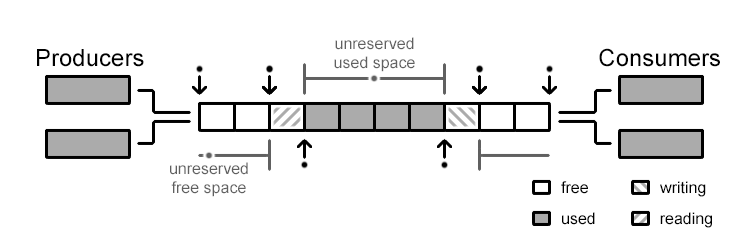
\includegraphics[width=0.80\textwidth]{images/ring.png}
    \caption{Struttura di un \textit{Ring Buffer}}
    \label{fig:ring_buffer}
\end{figure}

Le dimensioni dei ring buffer sono state calibrate sui worst case attesi:

\begin{itemize}
    \item \textbf{Board A, canale PC}: 8\,192 byte. Anche se l'immagine completa è di 36\,864 byte, l'applicazione consuma i byte in tempo reale via \texttt{read\_byte\_pc}, quindi il buffer accumula solo l'eventuale burst di byte arrivati tra una lettura e l'altra. 8~KB è un compromesso ampio.
    \item \textbf{Board A, canale b2b}: 256 byte. Sufficiente per le brevi risposte di tipo \texttt{TYPE\_TEXT} o \texttt{TYPE\_ACK} provenienti da Board B (poche decine di byte).
    \item \textbf{Board B, canale b2b}: 8\,199 byte. Pari a 8\,192 byte del crop più 7 byte di header del frame, in modo da poter assorbire un intero messaggio anche se l'applicazione fosse momentaneamente impegnata.
\end{itemize}

\section{Formato del frame}
\label{sec:frame-format}
Su un canale seriale orientato a flusso di byte, è necessario un protocollo di livello applicativo per delimitare i messaggi e identificarne il tipo. Il protocollo adottato in questo progetto utilizza un frame a lunghezza fissa di 7 byte di intestazione seguito da un payload di lunghezza variabile, come mostrato in Figura \ref{fig:protocollo}.

\begin{figure}[H]
    \centering
    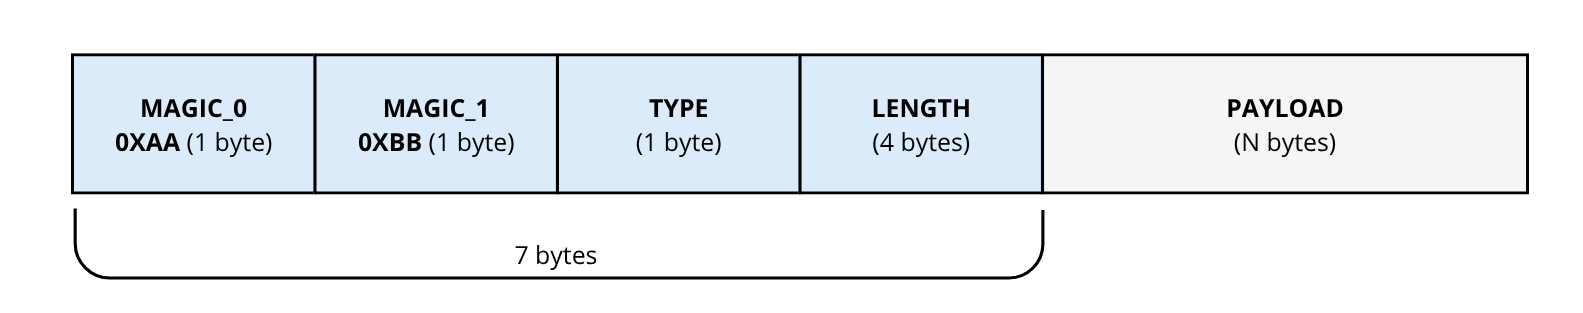
\includegraphics[width=0.95\textwidth]{images/protocollo_comunicazione.png}
    \caption{Struttura di un frame del protocollo applicativo}
    \label{fig:protocollo}
\end{figure}



I primi due byte (\textit{magic number}) costituiscono una sequenza di sincronizzazione: in ricezione, il parser scarta tutti i byte ricevuti finché non incontra la coppia $\mathtt{0xAA\,0xBB}$, dopodiché interpreta il byte successivo come tipo di messaggio. Il campo \texttt{TYPE}, di un singolo byte, identifica la natura del payload secondo la tabella dei tipi definiti per il protocollo (Tabella~\ref{tab:msg-types}). Il campo \texttt{LENGTH}, di 4 byte in \textit{big-endian}, indica la dimensione del payload che segue.

\begin{table}[H]
    \centering
    \caption{Tipi di messaggio definiti dal protocollo.}
    \label{tab:msg-types}
    \begin{tabular}{clll}
        \toprule
        \textbf{Codice} & \textbf{Nome} & \textbf{Direzione} & \textbf{Significato} \\
        \midrule
        $\mathtt{0x01}$ & \texttt{TYPE\_GRAY} & PC $\rightarrow$ A & Immagine grayscale da analizzare \\
        $\mathtt{0x02}$ & \texttt{TYPE\_BBOX} & A $\rightarrow$ PC & Bounding box (riservato, non usato) \\
        $\mathtt{0x03}$ & \texttt{TYPE\_ACK}  & A $\rightarrow$ PC, B $\rightarrow$ A & Sistema pronto \\
        $\mathtt{0x04}$ & \texttt{TYPE\_ERR}  & varie & Notifica di errore (codice in payload) \\
        $\mathtt{0x05}$ & \texttt{TYPE\_NONE} & A $\rightarrow$ PC & Nessuna targa rilevata \\
        $\mathtt{0x06}$ & \texttt{TYPE\_CROP} & A $\rightarrow$ B & Crop della targa per OCR \\
        $\mathtt{0x07}$ & \texttt{TYPE\_TEXT} & B $\rightarrow$ A $\rightarrow$ PC & Stringa di caratteri riconosciuta \\
        \bottomrule
    \end{tabular}
\end{table}

\section{Implementazione dei primitivi}
\label{sec:primitivi}

L'invio e la ricezione di un frame sono incapsulate in due primitive simmetriche, \texttt{send\_msg\_on} e \texttt{recv\_msg\_on}, parametrizzate dalle funzioni di lettura/scrittura del canale specifico (PC o b2b). In invio, la primitiva scrive in sequenza i due magic byte, il tipo, i quattro byte di lunghezza e infine il payload (Listato~\ref{lst:send}). In ricezione, la routine cerca prima la coppia di magic, legge il tipo e la lunghezza, e infine legge esattamente \texttt{size} byte di payload nel buffer fornito dal chiamante.

\begin{lstlisting}[style=stileC, caption={Primitiva generica per l'invio di un frame.}, label={lst:send}]
static void send_msg_on(void (*wb)(uint8_t),
                        void (*wbuf)(const uint8_t *, uint32_t),
                        uint8_t type, const uint8_t *payload, uint32_t len)
{
    wb(MAGIC_0); wb(MAGIC_1); wb(type);
    wb((len >> 24) & 0xFF);
    wb((len >> 16) & 0xFF);
    wb((len >>  8) & 0xFF);
    wb( len        & 0xFF);
    if (payload && len > 0) wbuf(payload, len);
}
\end{lstlisting}

L'uso di due puntatori a funzione consente al firmware di Board A di gestire i due canali (PC e Board B) con la stessa logica, differenziandoli solo per le primitive di byte. Sono definite due macro \texttt{send\_msg\_pc} e \texttt{send\_msg\_b2b} che istanziano la primitiva con le funzioni corrette per ciascun canale.

\section{Sincronizzazione di boot}
\label{sec:sync-boot}

All'accensione, le due schede non sono in uno stato consistente: la Board B impiega circa 500~ms a inizializzare la rete neurale, mentre Board A potrebbe terminare la propria inizializzazione prima che B sia pronta a ricevere. Se in questo intervallo il PC inviasse un'immagine, la Board A potrebbe accettarla, eseguire l'inferenza YOLO e tentare di inoltrare il crop a una Board B non ancora pronta, con il rischio di bloccare l'intero sistema.

Per evitare questa condizione di gara, è stato implementato un meccanismo di \textit{handshake} a due livelli:

\begin{enumerate}
    \item All'avvio, Board B termina l'inizializzazione della propria rete OCR e invia immediatamente un messaggio \texttt{TYPE\_ACK} sulla USART2 verso Board A.
    \item Board A, dopo aver inizializzato a sua volta la rete YOLO, si mette in attesa bloccante di un messaggio dalla USART2. Solo quando riceve l'ACK da B, la Board A invia il proprio \texttt{TYPE\_ACK} al PC sulla USART3.
    \item Lo script Python sul PC attende il primo messaggio dalla porta seriale e procede solo dopo aver ricevuto \texttt{TYPE\_ACK}. A questo punto inizia il ciclo di invio delle immagini.
\end{enumerate}

In questo modo la prima immagine viene inviata solo quando entrambi i microcontrollori hanno completato il proprio bring-up. Il meccanismo si comporta correttamente anche se le due schede vengono accese in ordine arbitrario, perché il timing assoluto non conta: ciò che conta è l'ordine causale degli ACK lungo la catena B~$\rightarrow$~A~$\rightarrow$~PC.

\chapter{Risultati sperimentali}
\label{cap:risultati}

Al fine di valutare il comportamento del sistema nelle condizioni operative previste, sono stati condotti una serie di test sperimentali inviando alla Board A, tramite uno script Python, immagini di veicoli con targa visibile, sia di nazionalità italiana che straniera, così da verificare la generalizzazione della pipeline su formati differenti. È stato inoltre incluso un caso negativo, ovvero un'immagine priva di veicoli, per osservare la risposta del sistema in assenza di una targa rilevabile. Per ciascun test vengono riportati l'immagine di input e la stringa riconosciuta restituita dalla Board B. Oltre ai risultati qualitativi del riconoscimento, vengono discussi i dati relativi all'occupazione della memoria (Flash e RAM) dei firmware caricati sulle due schede, nonché i tempi di computazione end-to-end misurati sull'intera pipeline, dall'invio e ricezione dell'immagine alla restituzione della targa riconosciuta.

\section{Configurazione del test}
\label{sec:test-setup}

Lo script Python di test (\texttt{plate\_recognition.py}) carica una singola immagine da disco, la pre-elabora portandola a $192\times192$ pixel in scala di grigi, e la invia alla Board A in un frame \texttt{TYPE\_GRAY}. Il tempo end-to-end è misurato sul PC tra l'invio del frame e la ricezione della risposta finale, comprendendo dunque tutti i trasferimenti UART, le due inferenze e l'overhead di sincronizzazione tra le board. La temporizzazione è effettuata con \texttt{time.perf\_counter()} di Python, che garantisce risoluzione al microsecondo.

Le immagini di test sono state selezionate per coprire condizioni eterogenee: targhe inquadrate frontalmente e di lato, con diversi livelli di illuminazione. Il dataset comprende un'immagine di paesaggio senza alcun veicolo, deliberatamente inclusa per verificare il corretto comportamento del sistema in assenza di targhe (caso che dovrebbe attivare la risposta \texttt{TYPE\_NONE}).

\section{Occupazione di memoria}
\label{sec:memoria-occupazione}

Al termine della build di entrambi i firmware, il sistema di compilazione di Zephyr riporta l'occupazione delle sezioni di memoria nella tabella di sintesi del linker. La Tabella~\ref{tab:footprint} riassume i valori misurati, si tenga conto che per entrambe le board la memoria Flash totale è di 1~MB e la memoria RAM totale di 512~KB.

\begin{table}[H]
    \centering
    \begin{tabular}{lrrrr}
        \toprule
        \textbf{Board} & \textbf{Flash usato} & \textbf{\% Flash} & \textbf{RAM usata} & \textbf{\% RAM} \\
        \midrule
        Board A (detection) & 907{,}16~KB & 88{,}59~\% & 502{,}00~KB & 98{,}05~\% \\
        Board B (OCR)       & 812{,}23~KB & 79{,}32~\% & 384{,}63~KB & 75{,}12~\% \\
        \bottomrule
    \end{tabular}
    \caption{Occupazione di Flash e RAM dei due firmware}
    \label{tab:footprint}
\end{table}

\begin{figure}[H]
    \centering
    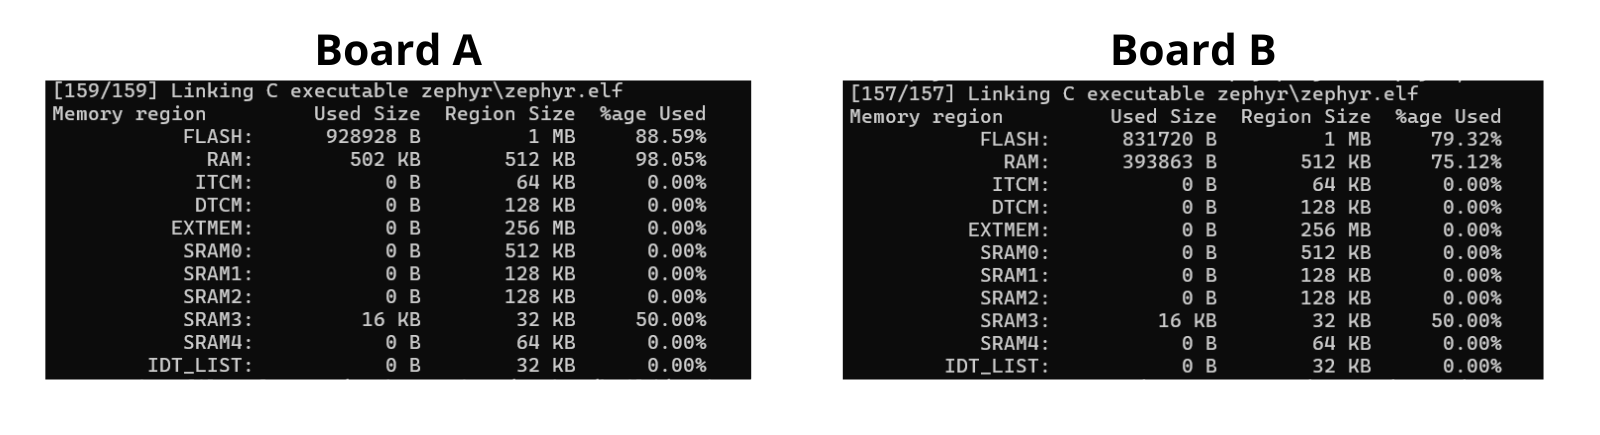
\includegraphics[width=0.95\textwidth]{images/occupazione_memoria_board.png}
    \caption{Output del linker Zephyr al termine della build dei due firmware}
    \label{fig:occupazione_memoria}
\end{figure}

Il dato più significativo è la quasi saturazione della RAM su Board A, a $98{,}05\,\%$ della capacità disponibile (502 KB su 512 KB, con appena 10 KB di margine residuo). Questo risultato non è casuale: l'occupazione è dominata dal solo buffer delle \textit{activation} della rete YOLO, che richiede 410\,112 byte ($\approx400$~KB). A questo si sommano l'\texttt{io\_buf} da 36\,864 byte, il \texttt{crop\_buf} da 8\,196 byte, i due ring buffer e il footprint statico del runtime Zephyr. Le ottimizzazioni descritte nei capitoli precedenti, in particolare l'uso della \texttt{union} per condividere lo stesso spazio tra l'immagine ricevuta e il tensore di input quantizzato, sono state necessarie per restare entro il budget disponibile. Sulla Board B la situazione è più rilassata: l'\textit{activation buffer} del CCT-XS richiede 296\,212 byte ($\approx289$~KB), inferiore di oltre 100~KB rispetto a quello di YOLO, e questo lascia un margine confortevole per il resto delle strutture dati. Anche l'occupazione di Flash è minore, perché il modello CCT-XS pesa circa 500~KB contro i 617~KB del modello YOLO.

Si può notare nella Figura \ref{fig:occupazione_memoria} che le regioni di memoria aggiuntive presenti sul microcontrollore, come ITCM, DTCM, SRAM0-4 ed EXTMEM, risultano inutilizzate in quanto il loro impiego richiederebbe un mapping esplicito nel linker script di Zephyr e un posizionamento manuale dei singoli buffer tramite attributi di sezione. Inoltre, strutture dati che per loro natura devono essere contigue in memoria,come i buffer di attivazione della rete neurale, non possono essere suddivise tra regioni fisicamente separate, rendendo di fatto impraticabile una distribuzione trasparente dei dati su più banchi. Per questi motivi, tutto il firmware è stato allocato nella regione RAM principale, che costituisce l'unica area di memoria gestita automaticamente da Zephyr.

\section{Risultati di riconoscimento}
\label{sec:risultati-riconoscimento}

Il sistema è in grado di riconoscere correttamente targhe italiane standard (formato $LL\,DDD\,LL$) ma anche straniere, a patto che siano presenti nel file di configurazione \texttt{.yaml} del relativo modello OCR presente nella repository utilizzata \cite{ankandrew_2024_fastplateocr}. \\
Sono stati condotti dei test utilizzando immagini di veicoli con targhe di nazionalità italiana, svizzera e tedesca, che differiscono tra loro per struttura, font e numero di caratteri. Di seguito, nelle Figure \ref{fig:riconoscimento_targhe_italiane} e \ref{fig:riconoscimento_targhe_straniere}, vengono riportati alcuni risultati rappresentativi: per ciascun caso è mostrata l'immagine originale che viene trasformata e inviata tramite lo script Python e il risultato finale di riconoscimento sotto forma di output nel terminale.

\begin{figure}[H]
    \centering
    % Prima riga
    \begin{subfigure}[t]{0.4\textwidth}
        \centering
        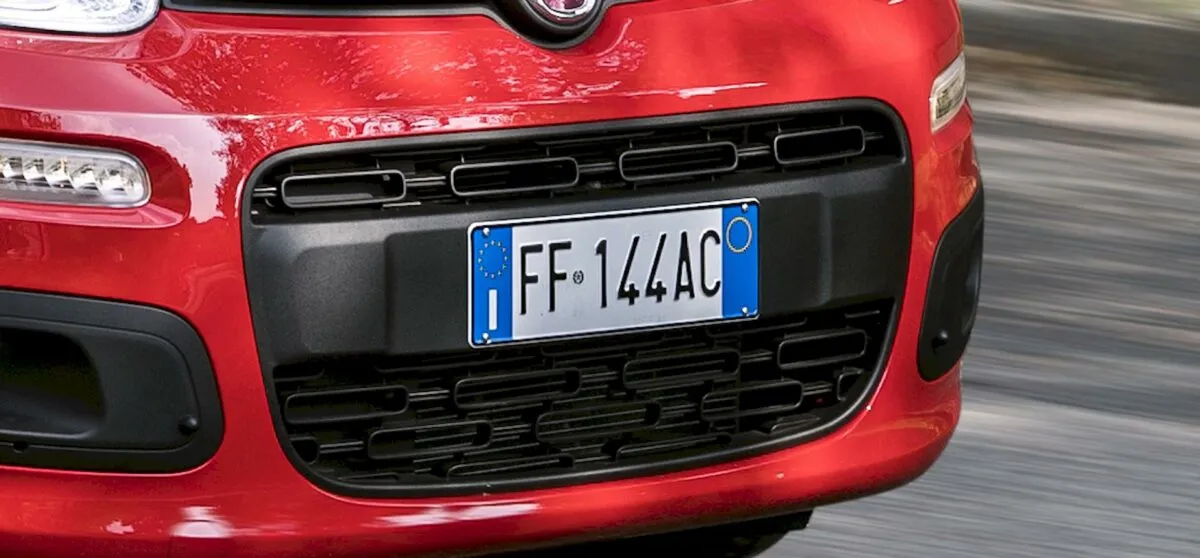
\includegraphics[width=\textwidth]{images/plate_25.png}
        \caption{Immagine originale}
        \label{fig:targa_originale_1}
    \end{subfigure}
    \hfill
    \begin{subfigure}[t]{0.59\textwidth}
        \centering
        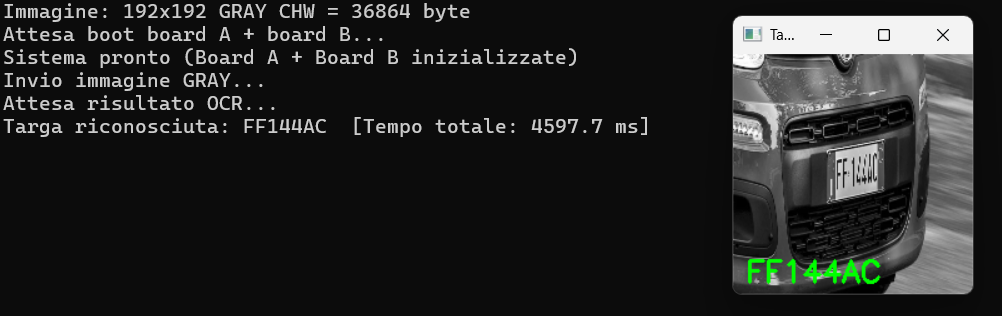
\includegraphics[width=\textwidth]{images/targa_italiana_riconosciuta.png}
        \caption{Output di riconoscimento della targa}
        \label{fig:output_targa_1}
    \end{subfigure}

    \vspace{0.5cm} % Spazio verticale tra le due righe

    % Seconda riga
    \begin{subfigure}[t]{0.4\textwidth} 
    \centering
    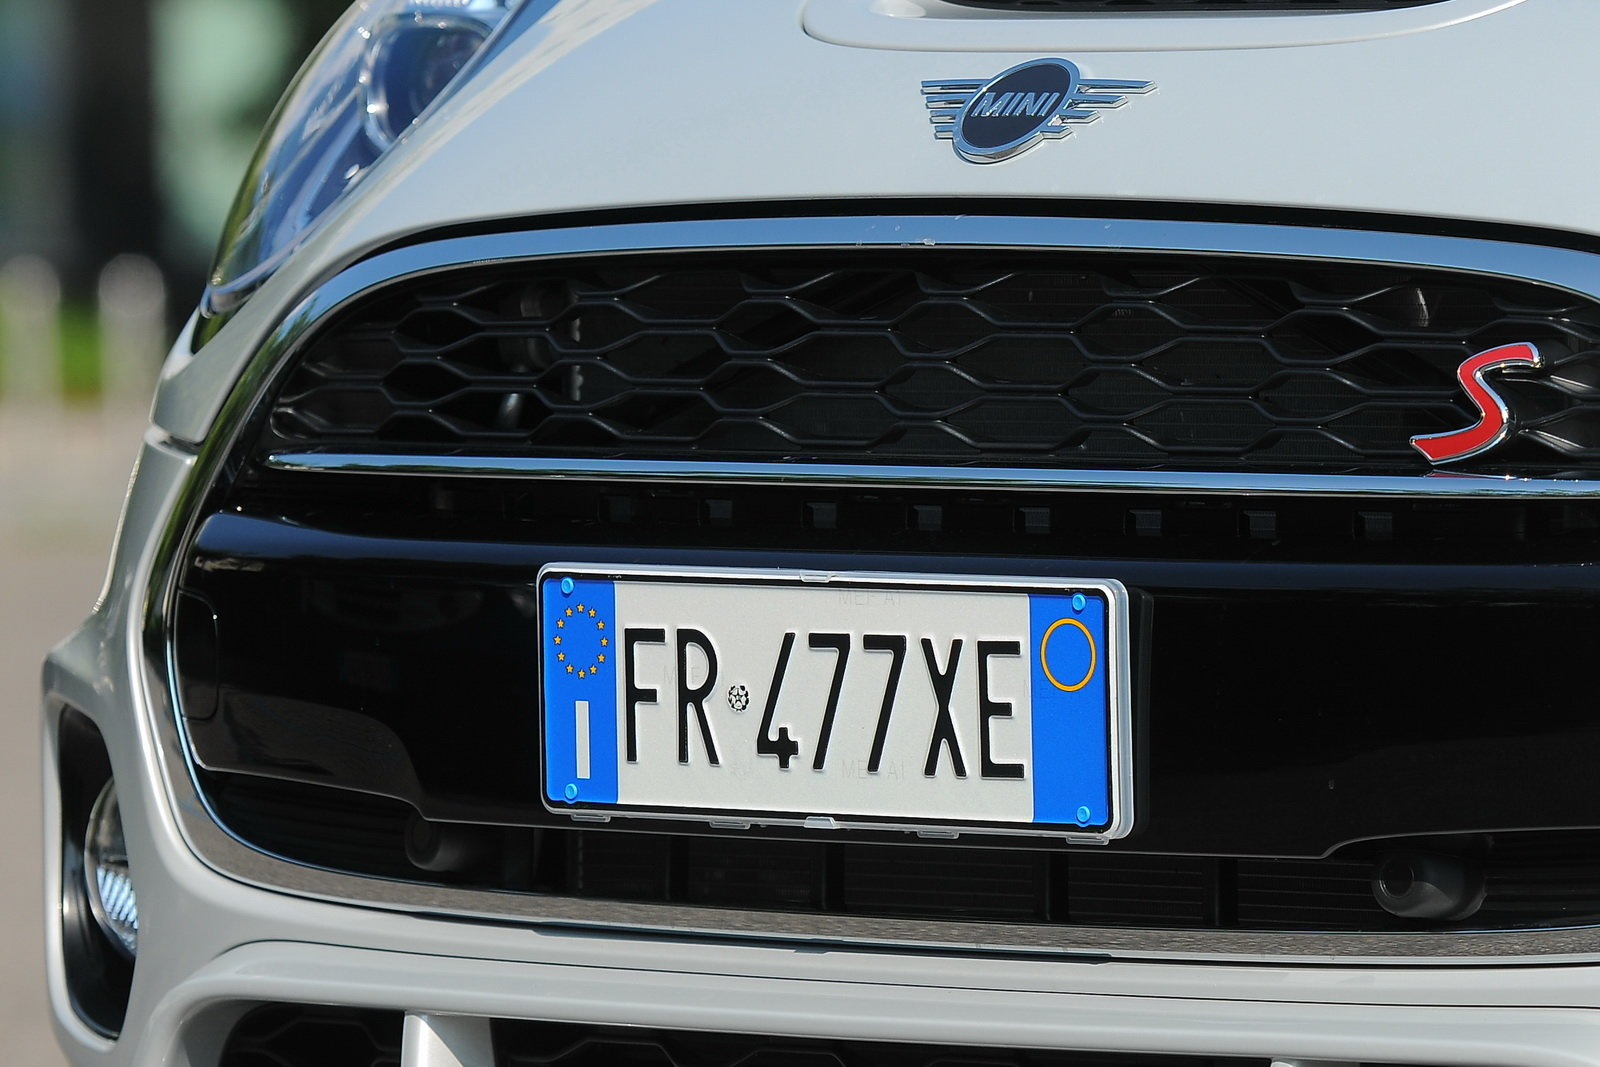
\includegraphics[
        width=\textwidth,
        trim=0 2cm 0 8cm,
        clip
    ]{images/plate_23.jpg}
    \caption{Immagine originale}
    \label{fig:targa_originale_2}
    \end{subfigure}
    \hfill
    \begin{subfigure}[t]{0.59\textwidth}
        \centering
        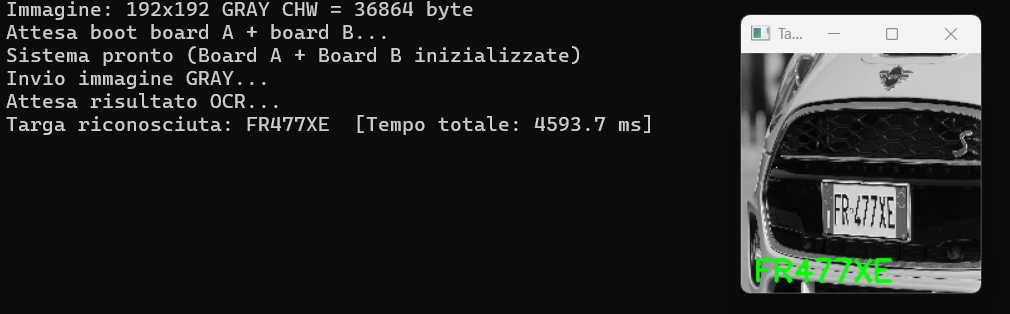
\includegraphics[width=\textwidth]{images/targa_italiana_riconosciuta_2.png}
        \caption{Output di riconoscimento della targa}
        \label{fig:output_targa_2}
    \end{subfigure}

    \caption{Esempi di riconoscimento corretto di targhe italiane}
    \label{fig:riconoscimento_targhe_italiane}
\end{figure}

\begin{figure}[H]
    \centering
    % Prima riga
    \begin{subfigure}[t]{0.4\textwidth}
        \centering
        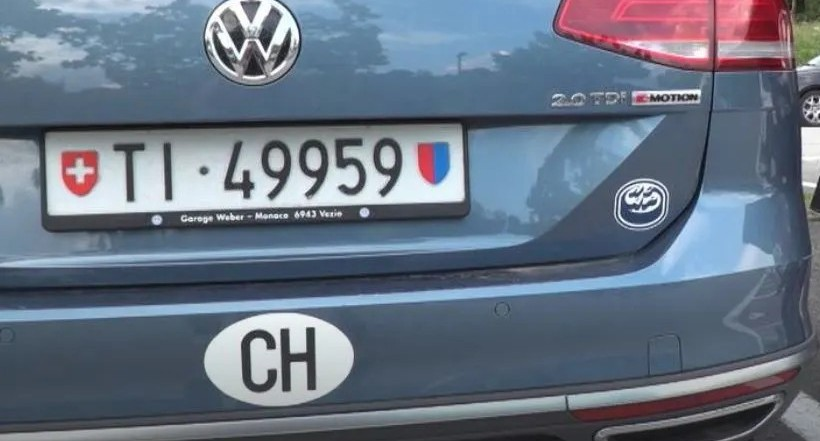
\includegraphics[width=\textwidth,
        trim=0 0 0 1.8cm,
        clip]{images/plate_21.jpg}
        \caption{Immagine originale}
        \label{fig:targa_originale_3}
    \end{subfigure}
    \hfill
    \begin{subfigure}[t]{0.59\textwidth}
        \centering
        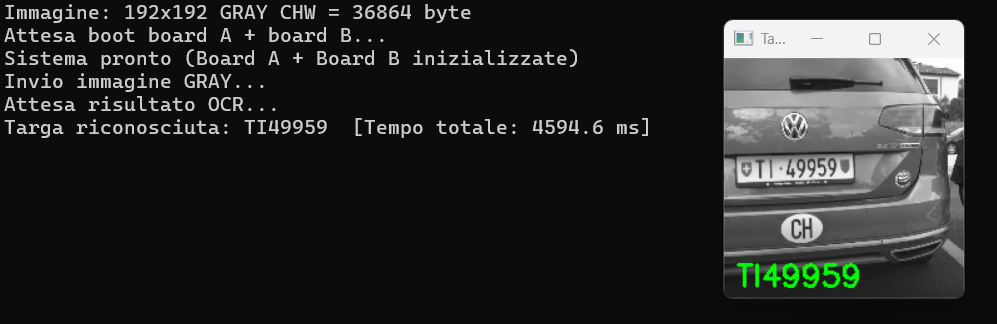
\includegraphics[width=\textwidth]{images/targa_svizzera_riconosciuta.png}
        \caption{Output di riconoscimento della targa}
        \label{fig:output_targa_3}
    \end{subfigure}

    \vspace{0.5cm} % Spazio verticale tra le due righe

    % Seconda riga
    \begin{subfigure}[t]{0.4\textwidth}
        \centering
        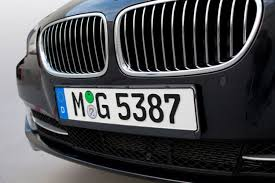
\includegraphics[width=\textwidth,
        trim=0 0 0 2cm,
        clip]{images/plate_14.jpg}
        \caption{Immagine originale}
        \label{fig:targa_originale_4}
    \end{subfigure}
    \hfill
    \begin{subfigure}[t]{0.59\textwidth}
        \centering
        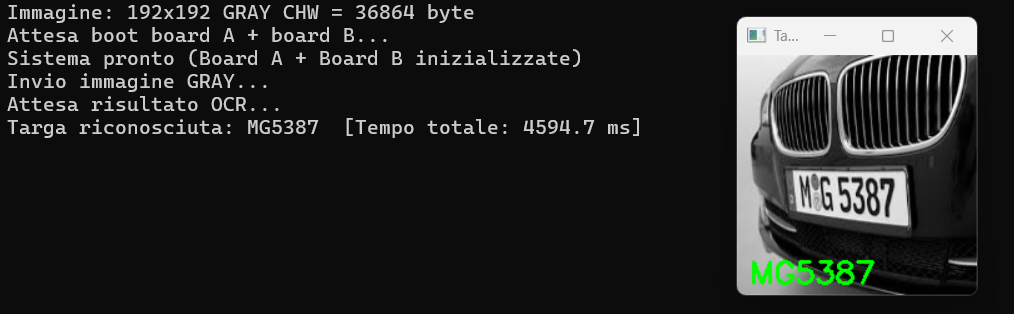
\includegraphics[width=\textwidth]{images/targa_tedesca_riconosciuta.png}
        \caption{Output di riconoscimento della targa}
        \label{fig:output_targa_4}
    \end{subfigure}

    \caption{Esempi di riconoscimento corretto di targe straniere (Svizzera e Germania)}
    \label{fig:riconoscimento_targhe_straniere}
\end{figure}

\subsection{Tempo end-to-end}
\label{sec:tempo-eed}

I tempi end-to-end misurati sulle quattro immagini precedente con detection riuscita sono riportati in Tabella~\ref{tab:tempi}. Il valore medio è di $4595{,}17$~ms con deviazione standard di $1{,}74$~ms: la latenza del sistema è dunque marcatamente deterministica, segno che l'esecuzione su Cortex-M7 senza task concorrenti non subisce variazioni di rilievo da un'esecuzione all'altra.

\begin{table}[H]
    \centering
    
    \begin{tabular}{lcc}
        \toprule
        \textbf{\#} & \textbf{Targa riconosciuta} & \textbf{Tempo (ms)} \\
        \midrule
        1 & FF144AC                   & 4597{,}7 \\
        2 & FR477XE                   & 4593{,}7 \\
        3 & TI49959                   & 4594{,}6 \\
        4 & MG5387                    & 4594{,}7 \\
        \midrule
        \multicolumn{2}{l}{\textit{Media}}   & $\mathbf{4595{,}17}$ \\
        \multicolumn{2}{l}{\textit{Std.dev.}} & $\mathbf{1{,}74}$ \\
        \bottomrule
    \end{tabular}
    \caption{Tempi end-to-end misurati su quattro immagini con detection riuscita}
    \label{tab:tempi}
\end{table}

\subsection{Analisi del bottleneck}
\label{sec:bottleneck}

La latenza di circa $4{,}6$~secondi è eccessiva per applicazioni in tempo reale, ed è utile capirne la composizione. Un calcolo a priori mostra che la sola trasmissione seriale è già il fattore dominante:

\begin{itemize}
    \item Il canale UART a 115\,200~baud con codifica 8N1 (10 bit per byte trasmesso, considerando bit di start e stop) sostiene un throughput utile di $11\,520$~byte/s.
    \item L'immagine $192\times192$ grayscale è di $36\,864$ byte, dunque la trasmissione PC~$\rightarrow$~A richiede $\approx3{,}20$~s.
    \item Il crop $128\times64$ è di $8\,192$ byte, dunque A~$\rightarrow$~B richiede $\approx0{,}71$~s.
\end{itemize}

La somma dei due trasferimenti seriali ammonta a circa 3,91 s, corrispondenti a circa l'85\% del tempo end-to-end osservato, evidenziando come il \textbf{collo di bottiglia principale} del sistema sia la comunicazione UART e non l'elaborazione neurale. I restanti $\approx680$~ms includono il tempo necessario per le due inferenze, insieme al post-processing, che comprende la Non-Maximum Suppression, la costruzione del crop, l'espansione da grayscale a RGB, la decodifica finale della targa e il sovraccarico legato alla sincronizzazione del protocollo.\\
È importante sottolineare che questo risultato va interpretato nel contesto sperimentale adottato: in una configurazione reale, il trasferimento iniziale dell'immagine dal PC alla Board A verrebbe infatti eliminato, sostituendo il PC con una videocamera direttamente collegata alla scheda. In tale scenario, la latenza complessiva si ridurrebbe sensibilmente, restando sostanzialmente limitata ai tempi di inferenza e post-processing sulla Board A e al trasferimento del crop verso la Board B, pari a circa 710 ms. Anche quest'ultimo contributo, tuttavia, può essere ulteriormente ridotto con interventi mirati, ad esempio aumentando il baud rate della comunicazione inter-board o adottando un'interfaccia più veloce come SPI.\\
Nel complesso, questi risultati mostrano che l'architettura distribuita proposta è solida e adatta a un impiego embedded autonomo e che i principali margini di miglioramento riguardano soprattutto il canale di comunicazione, più che la capacità di inferenza delle due schede.

\begin{boxH}
\textbf{In sintesi.} A 115\,200~baud, la sola trasmissione dei dati attraverso le UART occupa $\sim$3{,}9~s su 4{,}6~s di latenza totale. Le due inferenze, anche se impegnative per un Cortex-M7 senza acceleratore neurale, occupano nell'insieme meno del $15\,\%$ del tempo end-to-end, il che è un risultato ottimo.
\end{boxH}

\section{Validazione sul caso negativo}
Al fine di valutare la robustezza del sistema in assenza di un oggetto di interesse, è stato condotto un test inviando alla Board A un'immagine priva di veicoli e quindi priva di targhe rilevabili. L'obiettivo è verificare che la pipeline gestisca correttamente questo caso, rispondendo in modo appropriato senza produrre riconoscimenti errati o comportamenti inattesi. Il risultato di tale test si può osservare in Figura \ref{fig:riconoscimento_caso_negativo}.

\begin{figure}[H]
    \centering
    % Prima riga
    \begin{subfigure}[t]{0.34\textwidth}
        \centering
        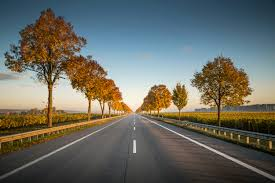
\includegraphics[width=\textwidth,
        trim=0 1cm 0 1.5cm,
        clip]{images/plate_26.jpg}
        \caption{Immagine originale}
        \label{fig:targa_originale_5}
    \end{subfigure}
    \hfill
    \begin{subfigure}[t]{0.65\textwidth}
        \centering
        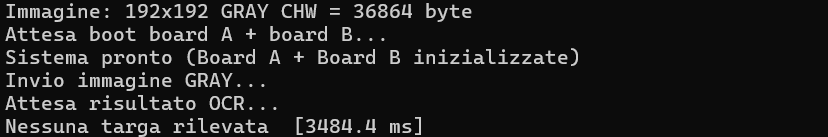
\includegraphics[width=\textwidth,
        trim=0 0 4cm 0,
        clip]{images/nessuna_targa.png}
        \caption{Output di riconoscimento della targa}
        \label{fig:output_targa_5}
    \end{subfigure}
    \caption{Esempio di riconoscimento del caso negativo: assenza di targhe}
    \label{fig:riconoscimento_caso_negativo}
\end{figure}
Il sistema, correttamente, produce una risposta \texttt{TYPE\_NONE} per cui nel log viene mostrata la frase "Nessuna targa rilevata". È interessante notare che il \textbf{tempo di risposta} è $\mathbf{3\,484{,}4}$~\textbf{ms}. Questo tempo è di circa $1\,100$~ms inferiore al caso con detection riuscita, e la differenza è esattamente quella attesa: viene a mancare il trasferimento del crop a Board~B (0{,}71~s) più la sua inferenza CCT e il viaggio di ritorno della stringa. Il caso è interessante perché conferma che il flusso di errori del protocollo funziona: in assenza di anchor sopra soglia, Board~A non tenta di forzare una predizione ma comunica esplicitamente al PC l'esito negativo.



\section{Analisi degli errori di riconoscimento}
\label{sec:errori}

In questa sezione vengono presentati alcuni casi in cui il sistema ha commesso errori di riconoscimento, al fine di analizzarne il comportamento in condizioni non ideali. I risultati riportati consentono di evidenziare le principali criticità emerse durante le prove sperimentali e di discutere le possibili cause degli errori osservati. Nella Figura \ref{fig:errori_riconoscimento_targhe_italiane} si possono notare due casi in cui è avvenuto un errore di riconoscimento delle targhe.

\begin{figure}[H]
    \centering
    % Prima riga
    \begin{subfigure}[t]{0.35\textwidth}
        \centering
        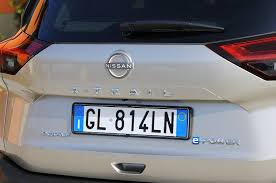
\includegraphics[width=\textwidth,
        trim=0 0 0 1cm,
        clip]{images/plate_2.jpg}
        \caption{Immagine originale}
        \label{fig:targa_originale_6}
    \end{subfigure}
    \hfill
    \begin{subfigure}[t]{0.64\textwidth}
        \centering
        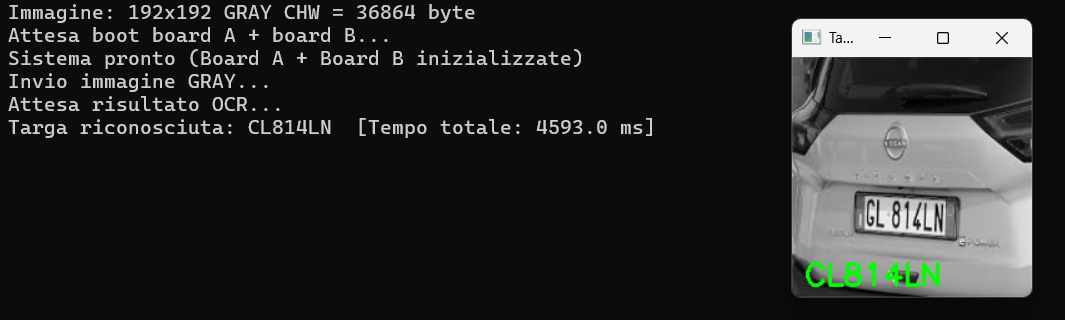
\includegraphics[width=\textwidth]{images/targa_italiana_errore2.png}
        \caption{Output di riconoscimento della targa}
        \label{fig:output_targa_6}
    \end{subfigure}

    \vspace{0.5cm} % Spazio verticale tra le due righe

    % Seconda riga
    \begin{subfigure}[t]{0.35\textwidth}
        \centering
        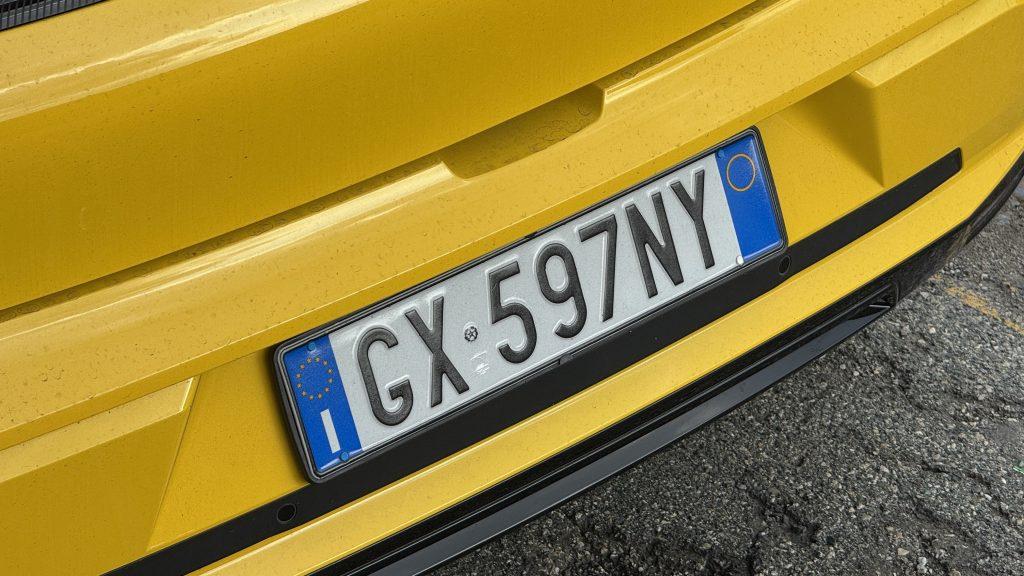
\includegraphics[width=\textwidth]{images/plate_4.jpg}
        \caption{Immagine originale}
        \label{fig:targa_originale_7}
    \end{subfigure}
    \hfill
    \begin{subfigure}[t]{0.64\textwidth}
        \centering
        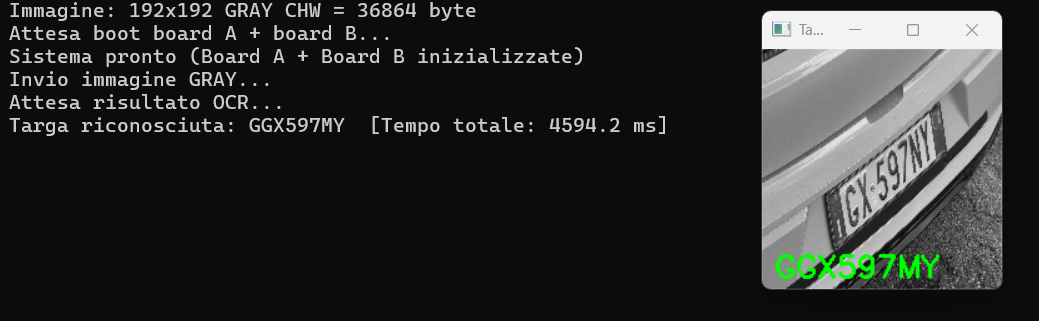
\includegraphics[width=\textwidth]{images/targa_italiana_errore1.png}
        \caption{Output di riconoscimento della targa}
        \label{fig:output_targa_7}
    \end{subfigure}

    \caption{Esempi di errori di riconoscimento in targhe italiane}
    \label{fig:errori_riconoscimento_targhe_italiane}
\end{figure}

Gli errori principali commessi dal sistema sono riconducibili ai seguenti:

\begin{itemize}
    \item \textbf{Slot duplicati}: nella Figura \ref{fig:output_targa_7}, la targa originale \texttt{GX597NY} viene letta come \texttt{GGX597MY}, con il primo carattere ripetuto. Si tratta di un'incertezza sull'allineamento spaziale dei caratteri all'interno della targa: il primo carattere si trova in una posizione che la rete fatica a discretizzare correttamente in uno dei 9 slot disponibili, e finisce per attivare due slot adiacenti. La causa di ciò è che, nell'immagine originale, la targa risulta inclinata e non perfettamente allineata orizzontalmente, rendendo più difficile la corretta segmentazione dei caratteri.
    \item \textbf{Confusione tra caratteri visivamente simili}: in entrambe le Figure (\ref{fig:output_targa_6} e \ref{fig:output_targa_7}) si nota questo errore. Nel primo caso, la targa originale \texttt{GL814LN} viene letta come \texttt{CL814LN}, con la \texttt{G} iniziale scambiata per \texttt{C}. Nel secondo caso, invece, la targa \texttt{GX597NY} viene riconosciuta come \texttt{GGX597MY}, mostrando sia la duplicazione del carattere iniziale (già discusso) sia l'errore sulla parte finale della stringa. Questi risultati evidenziano una limitazione tipica dei modelli OCR operanti a bassa risoluzione (in questo caso $128\times64$), dove caratteri visivamente simili possono essere confusi con maggiore facilità. La criticità può essere ulteriormente accentuata dal fatto che, quando il bounding box rilevato risulta più piccolo della risoluzione richiesta dalla rete OCR, viene applicato un upscaling dell'immagine: tale operazione, pur necessaria per adattare l'input al modello, può introdurre artefatti o amplificare differenze minime tra caratteri simili, contribuendo all'errore di classificazione.

\end{itemize}

Gli errori osservati dipendono soprattutto dalla \textbf{rete OCR pre-addestrata}, mentre YOLO individua in genere bounding box coerenti. Le criticità emergono nella lettura dei caratteri, specialmente con input difficili o a bassa risoluzione. In questi casi l'OCR può confondere simboli simili. Un possibile miglioramento consiste nel fine-tuning su un dataset più specifico.

\chapter{Conclusioni}
\label{cap:conclusioni}

\section{Riepilogo del lavoro svolto}
\label{sec:riepilogo}

In questo progetto è stato realizzato un sistema embedded distribuito per il riconoscimento automatico delle targhe, eseguito interamente su due microcontrollori STM32 Nucleo-H745ZI-Q comunicanti via UART. La distribuzione della pipeline ALPR su due schede è stata resa necessaria dai vincoli di memoria del singolo dispositivo e ha costituito al tempo stesso il principale obiettivo didattico del progetto. Le due reti sono state quantizzate e integrate in firmware Zephyr ottimizzati per l'uso della RAM disponibile, attraverso tecniche quali la condivisione di buffer tramite \texttt{union}, l'allocazione statica di tutte le strutture dati e la gestione interrupt-driven delle UART. Il sistema ha dimostrato di funzionare correttamente su un dataset di 26 immagini reali, riconoscendo targhe di paesi diversi con un tempo end-to-end di circa $4{,}6$~secondi e un'occupazione di RAM su Board~A pari al $98\,\%$ della capacità disponibile.

\section{Limitazioni}
\label{sec:limitazioni}

Le principali limitazioni del sistema riguardano tre aree distinte. Sul piano della \textbf{latenza}, il tempo end-to-end di \textbf{4,6~s} è dominato per l'$85\,\%$ dai trasferimenti UART a $115\,200$~baud (Sezione~\ref{sec:bottleneck}), non dall'inferenza; a questo si aggiunge il fatto che il sistema riceve immagini da un PC host anziché da una camera fisica, aggiungendo un trasferimento che in un'applicazione reale sarebbe eliminato. Sul piano delle \textbf{risorse hardware}, il margine residuo di circa $10$~KB di RAM su Board~A è estremamente sottile e qualsiasi estensione del firmware rischierebbe di superare la capacità disponibile; la mancanza di un acceleratore neurale dedicato (NPU) impone inoltre che l'intera inferenza sia svolta dal Cortex-M7, con tempi che non consentono un'elaborazione real-time. Sul piano dell'\textbf{accuratezza}, il modello CCT-XS occasionalmente confonde caratteri visivamente simili (\texttt{G}/\texttt{C}, \texttt{0}/\texttt{O}) o duplica slot adiacenti, limitazioni intrinseche della rete a bassa risoluzione non risolvibili lato firmware.

\section{Sviluppi futuri}
\label{sec:sviluppi-futuri}

\paragraph{Canale ad alta velocità.} La modifica con il maggior impatto sulla latenza è la sostituzione della UART con SPI a $8$~Mbps per il canale board-to-board, che ridurrebbe il trasferimento del crop da $710$~ms a meno di $10$~ms. Alzare il baud rate del canale PC$\leftrightarrow$Board~A a $921\,600$ porterebbe la trasmissione dell'immagine da $3{,}2$~s a $400$~ms.

\paragraph{Acquisizione diretta da camera.} L'interfaccia DCMI della H745 consente l'acquisizione da sensore di immagine in modalità DMA, eliminando completamente il trasferimento PC$\rightarrow$Board~A e rendendo il sistema autonomo rispetto all'host.

\paragraph{Migrazione a STM32N6.} La serie STM32N6 integra la NPU Neural-ART, che consentirebbe di eseguire entrambi i modelli su una singola scheda con tempi di inferenza di due ordini di grandezza inferiori, eliminando la comunicazione board-to-board e rendendo possibile l'elaborazione real-time.

\paragraph{Fine-tuning dell'OCR e gestione multi-targa.} Un ulteriore addestramento del CCT-XS su un dataset di targhe italiane ridurrebbe gli errori di confusione tra caratteri. Parallelamente, modificare la NMS per conservare tutte le detection sopra soglia permetterebbe di gestire scene con più veicoli, invocando Board~B una volta per ciascun crop rilevato.

\paragraph{Sfruttamento del dual-core.} Il core Cortex-M4 della H745, attualmente inutilizzato, potrebbe occuparsi della gestione delle UART e del protocollo, lasciando il M7 dedicato all'inferenza e abilitando il pipelining tra ricezione e calcolo.

% =====================================================================
%  Bibliografia
% =====================================================================
\bibliographystyle{ieeetr}
\bibliography{bibl}

\end{document}
